The following is part of latex file. Please translate this into R markdown. \setcounter{chapter}{2}
\chapter{Multiple Linear Regression - I}

{\small \textit{Chapter Preview}. This chapter introduces linear
regression in the case of several explanatory variables, known as
\emph{multiple linear regression}. Many basic linear regression
concepts extend directly, including goodness of fit measures such as
$R^2$ and inference using $t$-statistics. Multiple linear regression
models provide a framework for summarizing highly complex,
multivariate data. Because this framework requires only linearity in
the parameters, we are able to fit models that are nonlinear
functions of the explanatory variables, thus providing a wide scope
of potential applications.}

\section{Method of Least Squares}\label{S3:LSMethod}\index{least squares!method}

Chapter 2 dealt with the problem of a response depending on a single
explanatory variable. We now extend the focus of that chapter and study how
a response may depend on several explanatory variables.

\linejed

\empexjed{TermLife}\index{datasets!term life
insurance}\index{actuarial \& financial terms and concepts!demand}

\textbf{Example: Term Life Insurance.}\ecaptionjed{Demand for Term
Life Insurance} Like all firms, life insurance companies continually
seek new ways to deliver products to the market. Those involved in
product development wish to know ``who buys insurance and how much
do they buy?'' In economics, this is known as \emph{demand} side of
a market for products. Analysts can readily get information on
characteristics of current customers through company databases.
Potential customers, those that do not have insurance with the
company, are often the main focus for expanding market share.

In this example, we examine the Survey of Consumer Finances (SCF), a
nationally representative sample that contains extensive information
on assets, liabilities, income, and demographic characteristics of
those sampled (potential U.S. customers). We study a random sample
of 500 households with positive incomes that were interviewed in the
2004 survey. We initially consider the subset of $n=275$ families
that purchased term life insurance. We wish to address the second
portion of the demand question and determine family characteristics
that influence the amount of insurance purchased. Chapter 11 will
consider the first portion, whether or not a household purchases
insurance, through models where the response is a binary random
variable.

For term life insurance, the quantity of insurance is measured by
the policy FACE, the amount that the company will pay in the event
of the death of the named insured. Characteristics that will turn
out to be important include annual INCOME, the number of years of
EDUCATION of the survey respondent and the number of household
members, NUMHH.


\linejed\index{symbols!$k$, number of explanatory variables}

In general, we will consider data sets where there are $k$
explanatory variables and one response variable in a sample of size
$n$. That is, the data consist of:

\begin{center}
\begin{equation*}
\left\{
\begin{tabular}{c}
$x_{11},x_{12},\ldots,x_{1k},y_1$ \\
$x_{21},x_{22},\ldots,x_{2k},y_2$ \\
\\
$x_{n1},x_{n2},\ldots,x_{nk},y_n$%
\end{tabular}%
\right\} .
\end{equation*}
\end{center}

\noindent The $i$th observation corresponds to the $i$th row,
consisting of $(x_{i1},x_{i2},\ldots,x_{ik},y_i)$. For this general
case, we take $k+1$ measurements on each entity. For the insurance
demand example, $k=3$ and the data
consists of $(x_{11},x_{12},x_{13}, y_1)$, \ldots , $%
(x_{275,1},x_{275,2},x_{275,3},y_{275})$. That is, we use four
measurements from each of the $n=275$ households.

\subsubsection*{Summarizing the Data}

\marginparjed{Begin the data analysis by examining each variable in
isolation of the others.}

We begin the data analysis by examining each variable in isolation
of the others. Table \ref{T3:FaceSumStats} provides basic summary
statistics of the four variables. For FACE and INCOME, we see that
the mean is much greater than the median, suggesting that the
distribution is skewed to the right. Histograms (not reported here)
show that this is the case. It will turn out to be useful to also
consider their logarithmic transforms, LNFACE and LNINCOME,
respectively, that are also reported in Table \ref{T3:FaceSumStats}.

\begin{table}[h]
\caption{\label{T3:FaceSumStats} Term Life Summary Statistics}
\begin{center}
\begin{tabular}{lrrrrr}
\hline
                     &  & & Standard &  &  \\
Variable & Mean & Median & Deviation & Minimum & Maximum \\
\hline
      FACE &    747,581 &    150,000 &  1,674,362 &        800 & 14,000,000 \\
    INCOME &    208,975 &     65,000 &    824,010 &        260 & 10,000,000 \\
 EDUCATION &     14.524 &     16.000 &      2.549 &      2.000 &     17.000 \\
     NUMHH &      2.960 &      3.000 &      1.493 &      1.000 &      9.000 \\
    LNFACE &     11.990 &     11.918 &      1.871 &      6.685 &     16.455 \\
  LNINCOME &     11.149 &     11.082 &      1.295 &      5.561 &     16.118 \\
\hline
\end{tabular}\end{center}\end{table}

The next step is to measure the relationship between each $x$ on
$y$, beginning with the scatter plots in Figure
\ref{F3:TermLifeTwoPlots}. The left-hand panel is a plot of FACE
versus INCOME; with this panel, we see a large clustering in the
lower left-hand corner corresponding to households that have both
small incomes and face amounts of insurance. Both variables have
skewed distributions and their joint effect is highly nonlinear. The
right-hand panel presents the same variables but using logarithmic
transforms. Here, we see a relationship that can be more readily
approximated with a line.


\begin{figure}[htp]
  \begin{center}
 %     \includegraphics[width=2.5in,height=5in,angle=270]{Chapter3/F3TermLifeTwoPlotsB.ps}
    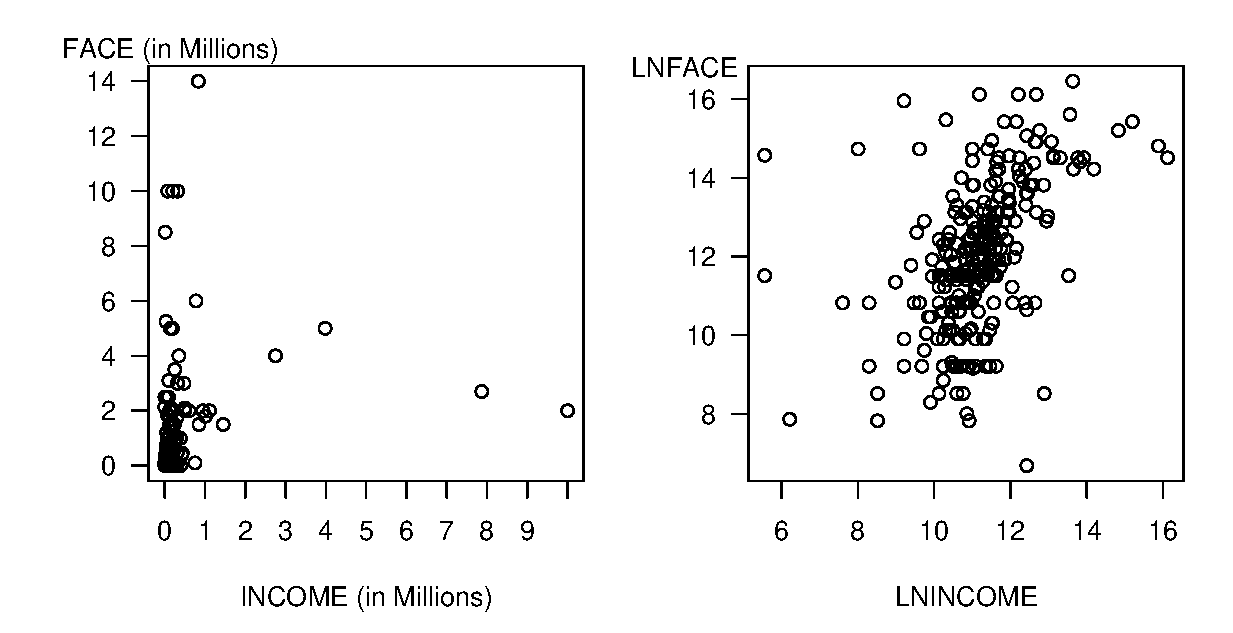
\includegraphics[width=.8\textwidth]{Chapter3/F3TermLifeTwoPlots.eps}
    \caption{\label{F3:TermLifeTwoPlots} \small  Income versus Face Amount of Term Life Insurance. The
left-panel is a plot of face versus income, showing a highly
nonlinear pattern. In the right-hand panel, face versus income is in
natural logarithmic units, suggesting a linear (although variable)
pattern.}
  \end{center}
\end{figure}

The Term Life data are \emph{multivariate} in the sense that several
measurements are taken on each household. It is difficult to produce
a graph of observations in three or more dimensions on a
two-dimensional platform, such as a piece of paper, that is not
confusing, misleading or both. To summarize graphically multivariate
data in regression applications, consider using a \emph{scatterplot
matrix} such as in Figure \ref{F3:TermLifeSMatrix}. Each square of
this figure represents a simple plot of one variable versus another.
For each square, the row variable gives the units of the vertical
axis and the column variable gives the units of the horizontal axis.
The matrix is sometimes called a \emph{half scatterplot matrix}
because only the lower left-hand elements are presented.

\begin{figure}[htp]
  \begin{center}
    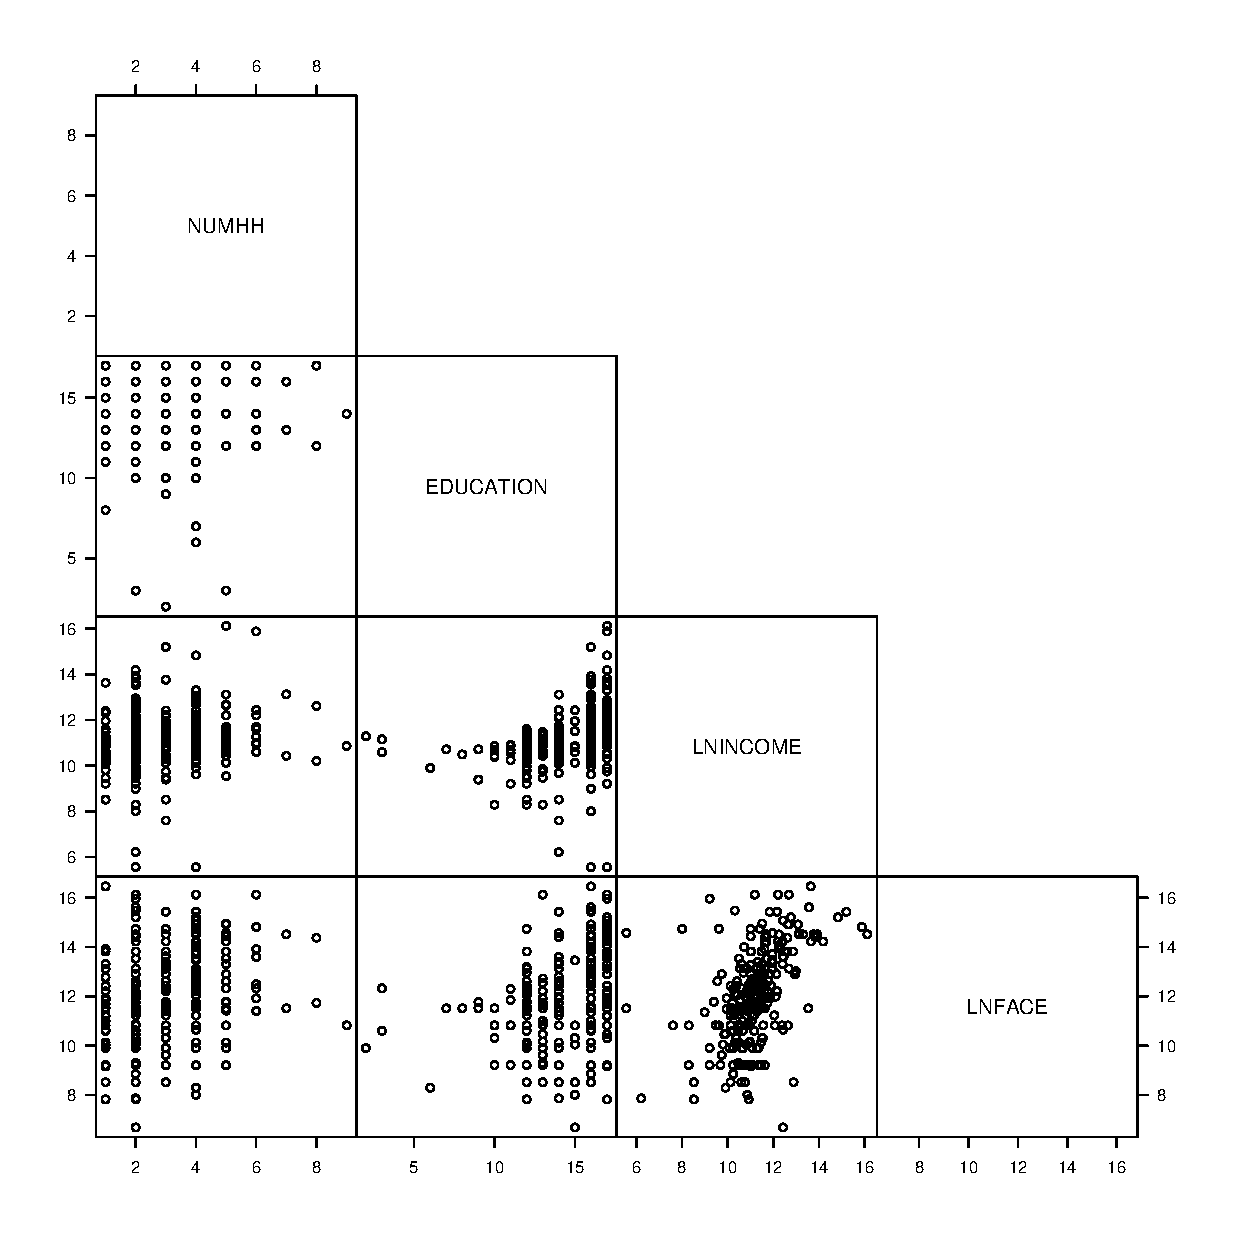
\includegraphics[width=1\textwidth]{Chapter3/F3TermLifeSMatrix.eps}
    \caption{\label{F3:TermLifeSMatrix} \small  Scatterplot
matrix of four variables. Each square is a scatter plot.}
  \end{center}
\end{figure}\index{plots!scatterplot matrix}\index{plots!half scatterplot matrix}

The scatterplot matrix can be numerically summarized using a
correlation matrix. Each correlation in Table \ref{T3:Corr}
corresponds to a square of the scatterplot matrix in Figure
\ref{F3:TermLifeSMatrix}. Analysts often present tables of
correlations because they are easy to interpret. However, remember
that a correlation coefficient merely measures the extent of linear
relationships. Thus, a table of correlations provides a sense of
linear relationships but may miss a nonlinear relationship that can
be revealed in a scatterplot matrix.




\begin{table}[h]
\caption{\label{T3:Corr} Term Life Correlations}
\begin{tabular}{lccc}
\hline
          &  NUMHH    & EDUCATION & LNINCOME  \\
EDUCATION & -0.064~   \\
LNINCOME  & 0.179     & 0.343   \\
LNFACE    & 0.288     & 0.383   & 0.482     \\

\hline
\end{tabular}\end{table}

The scatterplot matrix and corresponding correlation matrix are
useful devices for summarizing multivariate data. They are easy to
produce and to interpret. Still, each device captures only
relationships between pairs of variables and cannot quantify
relationships among several variables.

\subsubsection*{Method of Least Squares}

Consider the question: ``Can knowledge of education, household size
and income help us understand the demand for insurance?'' The
correlations in Table \ref{T3:Corr} and the graphs in Figures
\ref{F3:TermLifeTwoPlots} and \ref{F3:TermLifeSMatrix} suggest that
each variable, EDUCATION, NUMHH and LNINCOME, may be a useful
explanatory variable of LNFACE when taken individually. It seems
reasonable to investigate the \emph{joint} effect of these variables
on a response.

The geometric concept of a \emph{plane} is used to explore the
linear relationship between a response and several explanatory
variables. Recall that a plane extends the concept of a line to more
than two dimensions. A plane may be defined through an algebraic
equation such as
\begin{equation*}
y = b_0 + b_1 x_1 + \ldots + b_k x_k.
\end{equation*}
This equation defines a plane in $k+1$ dimensions. Figure
\ref{F3:3DPlane} shows a plane in three dimensions. For this figure,
there is one response variable, LNFACE, and two explanatory
variables, EDUCATION and LNINCOME (NUMHH is held fixed). It is
difficult to graph more than three dimensions in a meaningful way.

\begin{figure}[htp]
  \begin{center}
    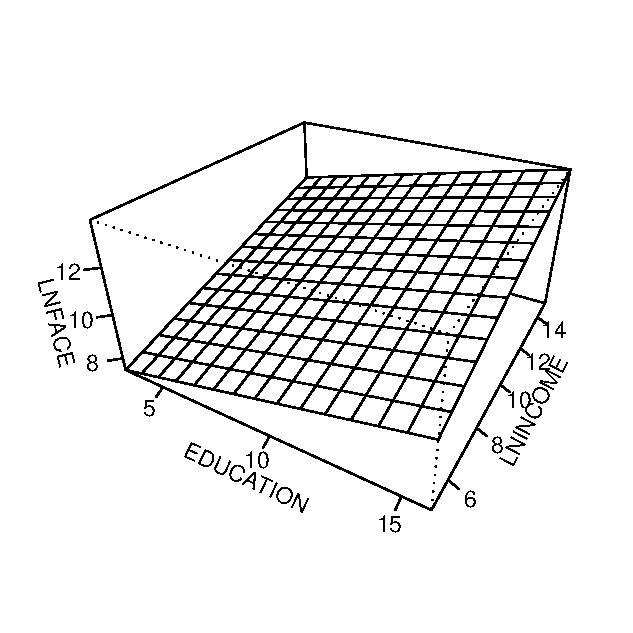
\includegraphics[width=.5\textwidth]{Chapter3/F33DPlane.eps}
    \caption{\label{F3:3DPlane} \small  An example of a three-dimensional plane.}
  \end{center}
\end{figure}

We need a way to determine a plane based on the data. The difficulty
is that in most regression analysis applications, the number of
observations, $n$, far exceeds the number of observations required
to fit a plane, $k+1$. Thus, it is generally not possible to find a
single plane that passes through all $n$ observations. As in Chapter
2, we use the \emph{method of least squares} to determine a plane
from the data.

The method of least squares is based on determining the values of $
b_0^{\ast},b_1^{\ast},\ldots,b_k^{\ast}$ that minimize the quantity
\begin{equation}\label{E3:SSBasic}
SS(b_0^{\ast},b_1^{\ast},\ldots,b_k^{\ast})=\sum_{i=1}^{n}\left(
y_i-\left(
b_0^{\ast}+b_1^{\ast}x_{i1}+\ldots+b_k^{\ast}x_{ik}\right) \right)
^2.
\end{equation}
We drop the asterisk, or star, notation and use $b_0, b_1, \ldots,
b_k$ to denote the best values, known as the \emph{least squares
estimates}. With the least squares estimates, define the \emph{least
squares, or fitted, regression plane} as
\begin{equation*}
\widehat{y} = b_0 + b_1 x_1 + \ldots + b_k x_k.
\end{equation*}\index{least
squares!regression plane}\index{symbols!$b_0, b_1, \ldots, b_k$,
least squares regression coefficients}

The least squares estimates are determined by minimizing
$SS(b_0^{\ast},b_1^{\ast},\ldots,b_k^{\ast})$. It is difficult to
write down the resulting least squares estimators using a simple
formula unless one resorts to matrix notation. Because of their
importance in applied statistical models, an explicit formula for
the estimators is provided below. However, these formulas have been
programmed into a wide variety of statistical and spreadsheet
software packages. The fact that these packages are readily
available allows data analysts to concentrate on the ideas of the
estimation procedure instead of focusing on the details of the
calculation procedures.

As an example, a regression plane was fit to the Term Life data
where three explanatory variables, $x_1$ for EDUCATION, $x_2$ for
NUMHH and $x_3$ for LNINCOME, were used. The resulting fitted
regression plane is

\begin{equation}\label{E3:TermRegression}
\widehat{y} = 2.584 + 0.206 x_1 + 0.306 x_2 + 0.494 x_3.
\end{equation}


\subsubsection*{Matrix Notation}\index{symbols!$\mathbf{y}$, vector of dependent
variables}\index{symbols!$\mathbf{X}$, matrix of explanatory
variables}

Assume that the data are of the form
$(x_{i0},x_{i1},\ldots,x_{ik},y_i)$, where $i = 1, \ldots, n$. Here,
the variable $x_{i0}$ is associated with the ``intercept'' term. That
is, in most applications, we assume that $x_{i0}$ is identically
equal to 1 and thus need not be explicitly represented. However,
there are important applications where this is not the case and
thus, to express the model in general notation, it is included here.
The data are represented in matrix notation using


\begin{equation*}
\mathbf{y}=\left(
\begin{array}{l}
y_1 \\
y_2 \\
\multicolumn{1}{c}{\vdots} \\
y_n%
\end{array}%
\right) ~~~\mathrm{and}~~~\mathbf{X}=\left(
\begin{array}{cccc}
x_{10} & x_{11} & \cdots & x_{1k} \\
x_{20} & x_{21} & \cdots & x_{2k} \\
\vdots & \vdots & \ddots & \vdots \\
x_{n0} & x_{n1} & \cdots & x_{nk}%
\end{array}%
\right) .
\end{equation*}%
Here, \textbf{y} is the $n\times 1$ vector of responses and
\textbf{X} is the $n\times (k+1)$ matrix of explanatory variables.
We use the matrix algebra convention that lower and upper case bold
letters represent vectors and matrices, respectively. (If you need
to brush up on matrices, review Section 2.11.)

\linejed

\textbf{Example: Term Life Insurance - Continued.} Recall that $y$
represents the logarithmic face, $x_1$ for years of education, $x_2$
for number of household members and $x_3$ for logarithmic income.
Thus, there are $k=3$ explanatory variables and $n=275$ households.
The vector of responses and the matrix of explanatory variables are:

\scalefont{0.80}
\begin{equation*}
\mathbf{y}=\left(
\begin{array}{l}
y_1 \\
y_2 \\
\multicolumn{1}{c}{\vdots} \\
y_{275}%
\end{array}%
\right) =\left(
\begin{array}{c}
9.904 \\
11.775 \\
\vdots \\
9.210
\end{array}%
\right) ~~~\mathrm{and}~~~\mathbf{X}=\left(
\begin{array}{cccc}
1 & x_{11} & x_{12} & x_{13} \\
1 & x_{21} & x_{22} & x_{23}\\
\vdots & \vdots & \vdots &\vdots\\
1 & x_{275,1} & x_{275,2} & x_{275,3}%
\end{array}%
\right) =\left(
\begin{array}{cccc}
1 & 16 & 3  & 10.669\\
1 & 9 & 3 & 9.393\\
\vdots & \vdots & \vdots &\vdots\\
1 & 12 & 1 & 10.545%
\end{array}%
\right) .
\end{equation*}
\scalefont{1.25}


\noindent For example, for the first observation in the data set,
the dependent variable is $y_1$=9.904 (corresponding to
$\textrm{exp}(9.904)= \$ 20,000$), for a survey respondent with 16
years of education living in a household with 3 people with
logarithmic income of 10.669 ($\exp (10.669)= \$ 43,000)$.

\linejed

Under the least squares estimation principle, our goal is to choose
the coefficients $b_0^{\ast},b_1^{\ast},\ldots,b_k^{\ast}$ to
minimize the sum of squares function
$SS(b_0^{\ast},b_1^{\ast},\ldots,b_k^{\ast})$. Using calculus, we
return to equation (\ref{E3:SSBasic}), take partial derivatives with
respect to each coefficient and set these quantities equal to zero:
\begin{equation*}
\frac{\partial }{\partial
b_j^{\ast}}SS(b_0^{\ast},b_1^{\ast},\ldots,b_k^{\ast})=\sum_{i=1}^{n}\left(
-2x_{ij}\right) \left( y_i-\left(
b_0^{\ast}+b_1^{\ast}x_{i1}+\ldots+b_k^{\ast}x_{ik}\right) \right)
=0,~~~\mathrm{for}~~j=0,1,\ldots .,k.
\end{equation*}
This is a system of $k+1$ equations and $k+1$ unknowns that can be readily
solved using matrix notation, as follows.

We may express the vector of parameters to be minimized as
$\mathbf{b}^{\ast}=(b_0^{\ast},b_1^{\ast},\ldots,b_k^{\ast})^{\prime}$.
Using this,
the sum of squares can be written as $SS(\mathbf{b}^{\ast})=(\mathbf{y-Xb}%
^{\ast})^{\prime}(\mathbf{y-Xb}^{\ast}).$ Thus, in matrix form, the
solution to the minimization problem can be expressed as $(\partial
/\partial \mathbf{b}^{\ast})SS(\mathbf{b}^{\ast})=\mathbf{0}$. This
solution satisfies the \emph{normal equations}
\begin{equation}\label{E3:NormalEquations}
\mathbf{X^{\prime}Xb}=\mathbf{X}^{\prime}\mathbf{y}.
\end{equation}
Here, the asterisk notation (*) has been dropped to denote the fact that $%
\mathbf{b}=(b_0,b_1,\ldots,b_k)^{\prime}$ represents the best vector
of values in the
sense of minimizing $SS(\mathbf{b}^{\ast})$ over all choices of $\mathbf{b}%
^{\ast}$.\index{symbols!$\mathbf{b}$, vector of regression
coefficients}\index{normal equations}

The least squares estimator $\mathbf{b}$ need not be unique.
However, assuming that the explanatory variables are not linear
combinations of one another, we have that $\mathbf{X^{\prime}X}$ is
invertible. In this case, we can write the unique solution as
\begin{equation}\label{E3:LSEstimates}
\mathbf{b}=\left( \mathbf{X^{\prime}X}\right) ^{-1}\mathbf{X}^{\prime}%
\mathbf{y}.
\end{equation}

\noindent To illustrate, for the Term Life example, equation
(\ref{E3:TermRegression}) yields
\begin{equation*}
\mathbf{b} = \left(
\begin{array}{c}
b_0 \\ b_1 \\ b_2 \\ b_3 \\
\end{array}
\right) = \left(
\begin{array}{c}
2.584 \\ 0.206 \\ 0.306 \\ 0.494 \\
\end{array}
\right).
\end{equation*}

\section{Linear Regression Model and Properties of Estimators}

In the previous section, we learned how to use the method of least
squares to fit a regression plane with a data set. This section
describes the assumptions underpinning the regression model and some
of the resulting properties of the regression coefficient
estimators. With the model and the fitted data, we will be able to
draw inferences about the sample data set to a larger population.
Moreover, we will later use these regression model assumptions to
help us improve the model specification in Chapter 5.

\subsection{Regression Function}

Most of the assumptions of the multiple linear regression model will
carry over directly from the basic linear regression model
assumptions introduced in Section 2.2. The primary difference is
that we now summarize the relationship between the response and the
explanatory variables through the \emph{regression
function}\index{regression function}

\begin{equation}\label{E3:MLRegressionFct}
\mathrm{E~}y=\beta_0 x_0+\beta_1 x_1+\ldots+\beta_k x_k,
\end{equation}%
that is linear in the parameters $\beta_0,\ldots ,\beta_k$.
Henceforth, we will use $x_0=1$ for the variable associated with the
parameter $\beta_0;$ this is the default in most statistical
packages and most applications of regression include the intercept
term $\beta_0$. The intercept is the expected value of $y$ when all
of the explanatory variables are equal to zero. Although rarely of
interest, the term $\beta_0$ serves to set the height of the fitted
regression plane.

\marginparjed{Interpret $\beta_j$ to be the expected change in $y$
per unit change in $x_j$ assuming all other explanatory variables
are held fixed.}\index{symbols!$\beta_j$, regression coefficient
associated with $x_j$}

In contrast, the other betas are typically important parameters from
a regression study. To help interpret them, we initially assume that
$x_j$ varies continuously and is not related to the other
explanatory variables. Then, we can interpret $\beta_j$ as the
expected change in $y$ per unit change in $x_j$ \emph{assuming all
other explanatory variables are held fixed}. That is, from calculus,
you will recognize that $\beta_j$ can be interpreted as a partial
derivative. Specifically, using equation (\ref{E3:MLRegressionFct}),
we have that
\begin{equation*}
\beta_j=\frac{\partial }{\partial x_j}\mathrm{E}~y.
\end{equation*}


\subsection{Regression Coefficient
Interpretation}\index{transformations!logarithmic}

Let us examine the regression coefficient estimates from the Term
Life Insurance example and focus initially on the \emph{sign} of the
coefficients. For example, from equation (\ref{E3:TermRegression}),
the coefficient associated with NUMHH is $b_2 = 0.306>0$. If we
consider two households that have the same income and the same level
of education, then the larger household (in terms of NUMHH) is
expected to demand \textit{more} term life insurance under the
regression model. This is a sensible interpretation, larger
households have more dependents for which term life insurance can
provide needed financial assets in the event of the untimely death
of a breadwinner. The positive coefficient associated with income
($b_3 = 0.494$) is also plausible; households with larger incomes
have more disposable dollars to purchase insurance. The positive
sign associated with EDUCATION ($b_1 = 0.206)$ is also reasonable,
more education suggests that respondents are more aware of their
insurance needs, other things being equal.

You will also need to interpret the \emph{amount} of the regression
coefficient. Consider first the EDUCATION coefficient. Using
equation (\ref{E3:TermRegression}), fitted values of
$\widehat{LNFACE}$ were calculated by allowing EDUCATION to vary and
keeping NUMHH and LNINCOME fixed at the sample averages. The results
are:
\begin{center}
\scalefont{0.9}
\begin{tabular}{lrrrr}
\hline \multicolumn{5}{c}{\textit{Effects of Small Changes in Education}} \\
\hline
 EDUCATION                &         14 &       14.1 &       14.2 &       14.3 \\
 $\widehat{LNFACE}$       &     11.883 &     11.904 &     11.924 &     11.945 \\
   $\widehat{FACE}$       &    144,803 &    147,817 &    150,893 &    154,034 \\
$\widehat{FACE}$ \% Change&            &      2.081 &      2.081 &      2.081 \\
\hline
\end{tabular}
\scalefont{1.1111}
\end{center}

\noindent As EDUCATION increases,  $\widehat{LNFACE}$ increases.
Further, the amount of $\widehat{LNFACE}$ increase is a constant
0.0206. This comes directly from equation (\ref{E3:TermRegression});
as EDUCATION increases by 0.1 years, we expect the demand for
insurance to increase by 0.0206 logarithmic dollars, holding NUMHH
and LNINCOME fixed. This interpretation is correct but most product
development directors are not overly fond of logarithmic dollars. To
return to dollars, fitted face values can be calculated through
exponentiation as $ \widehat{FACE}=\textrm{exp}(\widehat{LNFACE})$.
Moreover, the percentage change can be computed; for example,
$100*(147,817/144,803 - 1) \approx 2.08\% $. This provides another
interpretation of the regression coefficient; as EDUCATION increases
by 0.1 years, we expect the demand for insurance to increase by
2.08\%. This is a simple consequence of calculus using $ \partial
\textrm{ln} ~y /
\partial x  = \left(\partial y / \partial x \right) / y$; that is, a
small change in the logarithmic value of $y$ equals a small change
in $y$ as a proportion of $y$. It is because of this calculus result
that we use natural logs instead of common logs in regression
analysis. Because this table uses a discrete change in EDUCATION,
the 2.08\% differs slightly from the continuous result $0.206 \times
(\mathrm{change~in~EDUCATION}) = 2.06\%$. However, this proximity is
usually regarded as suitable for interpretation purposes.

Continuing this logic, consider small changes in logarithmic income.

\begin{center}
\scalefont{0.9}
\begin{tabular}{lrrrr}
\hline \multicolumn{5}{c}{\textit{Effects of Small Changes in Logarithmic Income}} \\
 \hline
  LNINCOME &         11 &       11.1 &       11.2 &       11.3 \\
    INCOME &     59,874 &     66,171 &     73,130 &     80,822 \\
INCOME \% Change  &            &      10.52 &      10.52 &      10.52 \\
\hline
 $\widehat{LNFACE}$ &     11.957 &     12.006 &     12.055 &     12.105 \\
 $\widehat{FACE}$ &    155,831 &    163,722 &    172,013 &    180,724  \\
$\widehat{FACE}$ \% Change &            &       5.06 &       5.06 &       5.06 \\
\hline
$\widehat{FACE}$ \% Change / INCOME \% Change &            &       0.482 &      0.482 &      0.482 \\
\hline
\end{tabular}
\scalefont{1.1111}
\end{center}

\index{actuarial \& financial terms and concepts!elasticity}


\noindent We can use the same logic to interpret the LNINCOME
coefficient in equation (\ref{E3:TermRegression}). As logarithmic
income increases by 0.1 units, we expect the demand for insurance to
increase by 5.06\%. This takes care of logarithmic units in the $y$
but not the $x$. We can use the same logic to say that as
logarithmic income increases by 0.1 units, INCOME increases by
10.52\%. Thus, a 10.52\% change in INCOME corresponds to a 5.06\%
change in FACE. Summarizing, we say that, holding NUMHH and
EDUCATION fixed, we expect that a 1\% increase in INCOME is
associated with a 0.482\% increase in $\widehat{FACE}$ (as before,
this is close to the parameter estimate $b_3 = 0.494$). The
coefficient associated with income is known as an \emph{elasticity}
in economics. In economics, elasticity is the ratio of the percent
change in one variable to the percent change in another variable.
Mathematically, we summarize this as
\begin{equation*}
\frac{\partial \textrm{ln} ~y}{\partial \textrm{ln} ~x} =
\left(\frac{\partial ~y}{y}\right)/\left(\frac{\partial
~x}{x}\right).
\end{equation*}

\subsection{Model Assumptions}\index{model assumptions!observables
representation}\index{model assumptions!error representation}

As in Section 2.2 for a single explanatory variable, there are two
sets of assumptions that one can use for multiple linear regression.
They are equivalents sets, each having comparative advantages as we
proceed in our study of regression. The ``observables''
representation focuses on variables of interest
$(x_{i1},\ldots,x_{ik},y_i).$ The ``error representation'' provides
a springboard for motivating our goodness of fit measures and study
of residual analysis. However, the latter set of assumptions focuses
on the additive errors case and obscures the sampling basis of the
model.


\scalefont{0.8}

\begin{center}
\begin{tabular}{cc}
\hline
\multicolumn{2}{c}{\large{Multiple Linear Regression Model Sampling Assumptions}} \\
Observables Representation & Error Representation \\ \hline
\multicolumn{1}{l}{F1. $\mathrm{E}~y_i=\beta_0+\beta_1
x_{i1}+\ldots+\beta_k x_{ik}$.} & \multicolumn{1}{l}{E1.
$y_i=\beta_0+\beta_1 x_{i1}+\ldots+\beta_k x_{ik}+\varepsilon_i$.} \\
\multicolumn{1}{l}{F2. $\{x_{i1},\ldots ,x_{ik}\}$} &
\multicolumn{1}{l}{E2.
$\{x_{i1},\ldots ,x_{ik}\}$} \\
are non-stochastic variables. & are non-stochastic variables. \\
\multicolumn{1}{l}{F3. $\mathrm{Var}~y_i=\sigma^2$.} &
\multicolumn{1}{l}{E3. $\mathrm{E}~\varepsilon_i=0$ and $\mathrm{Var}~\varepsilon_i=\sigma^2$.} \\
\multicolumn{1}{l}{F4. \{$y_i$\} are independent random variables.}
& \multicolumn{1}{l}{E4. \{$\varepsilon_i$\} are independent random
variables.} \\
\multicolumn{1}{l}{F5. \{$y_i$\} are normally distributed.} &
\multicolumn{1}{l}{E5. \{$\varepsilon_i$\} are normally distributed.} \\
\hline
\end{tabular}
\end{center}


\scalefont{1.25}

To further motivate Assumptions F2 and F4, we will usually assume
that our data have been realized as the result of a stratified
sampling scheme, where each unique value of
$\{x_{i1},\ldots,x_{ik}\}$ is treated as a stratum. That is, for
each value of $\{x_{i1},\ldots,x_{ik}\}$, we draw a random sample of
responses from a population. Thus, responses within each stratum are
independent from one another, as are responses from different
strata. Chapter 6 will discuss this sampling basis in further
detail.

\subsection{Properties of Regression Coefficient Estimators}
\index{symbols!$\boldsymbol \beta$, vector of regression
coefficients}

Section \ref{S3:LSMethod} described the least squares method for
estimating regression coefficients. With the regression model
assumptions, we can establish some basic properties of these
estimators. To do this, from Section 2.11.4 we have that the
expectation of a vector is the vector of expectations, so that
\begin{equation*}
\mathrm{E}~\mathbf{y}=\left(
\begin{array}{l}
\mathrm{E}~y_1 \\
\mathrm{E}~y_2 \\
\multicolumn{1}{c}{\vdots} \\
\mathrm{E}~y_n
\end{array}
\right) .
\end{equation*}
Further, basic matrix multiplication shows that
\begin{equation*}
\mathbf{X} \boldsymbol \beta=\left(
\begin{array}{cccc}
1 & x_{11} & \cdots & x_{1k} \\
1 & x_{21} & \cdots & x_{2k} \\
\vdots & \vdots & \ddots & \vdots \\
1 & x_{n,1} & \cdots & x_{n,k}%
\end{array}%
\right) \left(
\begin{array}{c}
\beta_0 \\
\beta_1 \\
\vdots \\
\beta_k%
\end{array}
\right) =\left(
\begin{array}{c}
\beta_0 + \beta_1 x_{11} + \cdots + \beta_k x_{1k} \\
\beta_0 + \beta_1 x_{21} + \cdots + \beta_k x_{2k} \\
\vdots \\
\beta_0 + \beta_1 x_{n1} + \cdots + \beta_k x_{nk}
\end{array}
\right) .
\end{equation*}
Because the $i$th row of assumption F1 is $\mathrm{E}~y_i = \beta_0
+ \beta_1 x_{i1} + \cdots + \beta_k x_{ik}$, we may re-write this
assumption in matrix formulation as
$\mathrm{E}~\mathbf{y}=\mathbf{X}\boldsymbol \beta$. We are now in a
position to state the first important property of least squares
regression estimators.

\bigskip

\boxedjed

\textbf{Property 1}. Consider a regression model and let Assumptions
F1-F4 hold. Then, the estimator $\mathbf{b}$ defined in equation
(\ref{E3:LSEstimates}) is an unbiased estimator of the parameter
vector $\boldsymbol \beta$.
\end{boxedminipage}\index{estimator!unbiased}

\bigskip

To establish Property 1, we have that

\begin{equation*}
\mathrm{E}~\mathbf{b} = \mathrm{E}~\left(
(\mathbf{X^{\prime}X)}^{-1}\mathbf{X}^{\prime}\mathbf{y}\right)
=(\mathbf{X^{\prime}X)}^{-1}\mathbf{X}^{\prime}\mathrm{E}~\mathbf{y}
=(\mathbf{X^{\prime}X)}^{-1} \mathbf{X}^{\prime} \left( \mathbf{X}
\boldsymbol \beta \right) = \boldsymbol \beta,
\end{equation*}
using matrix multiplication rules. This chapter assumes that
$\mathbf{X^{\prime}X}$ is invertible. One can also show that the
least squares estimator need only be a solution of the normal
equations for unbiasedness (not requiring that
$\mathbf{X^{\prime}X}$ be invertible, see Section 4.7.3). Thus,
$\mathbf{b}$ is said to be an \emph{unbiased estimator }of
$\boldsymbol \beta$. In particular, E $b_j$ = $\beta_j$ for $j =
0,1,\ldots,k$.

Because independence implies zero covariance, from Assumption F4 we
have that $\mathrm{Cov}(y_i,y_j)=0$ for $i\neq j$. From this,
Assumption F3 and the definition of the variance of a vector, we
have that
\begin{equation*}
\mathrm{Var~}\mathbf{y}=\left(
\begin{array}{cccc}
\mathrm{Var~}y_1 & \mathrm{Cov}(y_1,y_2) & \cdots & \mathrm{Cov}
(y_1,y_n) \\
\mathrm{Cov}(y_2,y_1) & \mathrm{Var~}y_2 & \cdots & \mathrm{Cov}
(y_2,y_n) \\
\vdots & \vdots & \ddots & \vdots \\
\mathrm{Cov}(y_n,y_1) & \mathrm{Cov}(y_n,y_2) & \cdots &
\mathrm{Var~ }y_n
\end{array}
\right) =\left(
\begin{array}{cccc}
\sigma^2 & 0 & \cdots & 0 \\
0 & \sigma^2 & \cdots & 0 \\
\vdots & \vdots & \ddots & \vdots \\
0 & 0 & \cdots & \sigma^2
\end{array}
\right) =\sigma^2\mathbf{I},
\end{equation*}
where $\mathbf{I}$\ is an an $n\times n$ identity matrix. We are now
in a position to state the second important property of least
squares regression estimators.
\bigskip

\boxedjed

\textbf{Property 2.} Consider a regression model and let Assumptions
F1-F4 hold. Then, the estimator $\mathbf{b}$ defined in equation
(\ref{E3:LSEstimates}) has variance $\mathrm{Var~}\mathbf{b}
=\sigma^2(\mathbf{X^{\prime}X)}^{-1}.$
\end{boxedminipage}
\bigskip

To establish Property 2, we have that

\begin{eqnarray*}
\mathrm{Var~}\mathbf{b} &=&\mathrm{Var}\left(
(\mathbf{X^{\prime}X)}^{-1} \mathbf{X}^{\prime}\mathbf{y}\right)
=\left[ (\mathbf{X^{\prime}X)}^{-1} \mathbf{X}^{\prime}\right]
\mathrm{Var}\left( \mathbf{y}\right) \left[
\mathbf{X}(\mathbf{X^{\prime}X)}^{-1}\right] \\
&=&\left[ (\mathbf{X^{\prime}X)}^{-1}\mathbf{X}^{\prime}\right]
\sigma^2 \mathbf{I}\left[
\mathbf{X}(\mathbf{X^{\prime}X)}^{-1}\right] =\sigma^2(
\mathbf{X^{\prime}X)}^{-1}\mathbf{X}^{\prime}\mathbf{X}(\mathbf{X^{\prime}X)}^{-1}=\sigma
^2(\mathbf{X^{\prime}X)}^{-1},
\end{eqnarray*}
as required. This important property will allow us to measure the
precision of the estimator $\mathbf{b}$ when we discuss statistical
inference. Specifically, by the definition of the variance of a
vector (see Section 2.11.4),
\begin{equation}\label{E3:VarVec}
\mathrm{Var~}\mathbf{b}=\left(
\begin{array}{cccc}
\mathrm{Var~}b_0 & \mathrm{Cov}(b_0,b_1) & \cdots & \mathrm{Cov}%
(b_0,b_k) \\
\mathrm{Cov}(b_1,b_0) & \mathrm{Var~}b_1 & \cdots & \mathrm{Cov}%
(b_1,b_k) \\
\vdots & \vdots & \ddots & \vdots \\
\mathrm{Cov}(b_k,b_0) & \mathrm{Cov}(b_k,b_1) & \cdots & \mathrm{Var~%
}b_k%
\end{array}
\right) =\sigma^2 (\mathbf{X^{\prime}X)}^{-1}.
\end{equation}
Thus, for example, $\mathrm{Var~}b_j$ is $\sigma^2$ times the
$(j+1)st$
diagonal entry of $(\mathbf{X^{\prime}X)}^{-1}$. As another example, $\mathrm{Cov}%
(b_0,b_j)$ is $\sigma^2$ times the element in the first row and $%
(j+1)st$ column of $(\mathbf{X^{\prime}X)}^{-1}$.

Although alternative methods are available that are preferable for
specific applications, the least squares estimators have proven to
be effective for many routine data analyses. One desirable
characteristic of least squares regression estimators is summarized
in the following well-known result.

\bigskip
\boxedjed\index{theorems!Gauss-Markov}

\textbf{Gauss-Markov Theorem.} Consider the regression model and let
Assumptions F1-F4 hold. Then, within the class of estimators that
are linear functions of the responses, the least squares estimator
$\mathbf{b}$ defined in equation (\ref{E3:LSEstimates}) is the
minimum variance unbiased estimator of the parameter vector
$\boldsymbol \beta$.
\end{boxedminipage}
\bigskip

\marginparjed{The Gauss-Markov theorem states that the least squares
estimator is the most precise in the sense that it has the smallest
variance.}

We have already seen in Property 1 that the least squares estimators
are unbiased. The Gauss-Markov theorem states that the least squares
estimator is the most precise in the sense that it has the smallest
variance. (In a matrix context, ``minimum variance'' means that if
$\mathbf{b}^{\ast}$ is any other estimator, then the difference of
the variance matrices, $\mathrm{Var~}
\mathbf{b}^{\ast}\mathbf{-}\mathrm{Var~}\mathbf{b}$, is nonnegative
definite.)

An additional important property concerns the distribution of the
least squares regression estimators.

\bigskip
\boxedjed

\textbf{Property 3}. Consider a regression model and let Assumptions
F1-F5 hold. Then, the least squares estimator $\mathbf{b}$ defined
in equation (\ref{E3:LSEstimates}) is normally distributed.
\end{boxedminipage}
\bigskip

\noindent To establish Property 3, we define the weight vectors,
$\mathbf{w}_i=(\mathbf{X^{\prime}X)}^{-1}\left( 1,x_{i1}, \ldots,
x_{ik}\right) ^{\prime}$. With this notation, we note that
\begin{equation*}
\mathbf{b=}(\mathbf{X^{\prime}X)}^{-1}\mathbf{X}^{\prime}\mathbf{y=}
\sum_{i=1}^{n}\mathbf{w}_iy_i,
\end{equation*}
so that $\mathbf{b}$ is a linear combination of responses. With
Assumption F5, the responses are normally distributed. Because
linear combinations of normally distributed random variables are
normally distributed, we have the conclusion of Property 3. This
result underpins much of the statistical inference that will be
presented in Sections 3.4 and 4.2.


\section{Estimation and Goodness of Fit}\index{goodness of fit
statistics}

\subsubsection*{Residual Standard Deviation}

Additional properties of the regression coefficient estimators will
be discussed when we focus on statistical inference. We now continue
our estimation discussion by providing an estimator of the other
parameter in the linear regression model, $\sigma^2$.

Our estimator for $\sigma^2$ can be developed using the principle of
replacing theoretical expectations by sample averages. Examining
$\sigma^2=\mathrm{E}\left( y-\mathrm{E~}y\right)^2$, replacing the
outer expectation by a sample average suggests using the estimator $
n^{-1}\sum_{i=1}^{n}(y_i-\mathrm{E~}y_i)^2$. Because we do not
observe $\mathrm{E}~y_i = \beta_0 + \beta_1 x_{i1} + \cdots +
\beta_k x_{ik}$, we use in its place the corresponding observed
quantity $b_0 + b_1 x_{i1}+\ldots+b_k x_{ik}=\widehat{y}_i$. This
leads to the following.


\bigskip

\boxedjed

\textit{Definition}. An estimator of $\sigma^2$, the \emph{mean
square error (MSE)}, is defined as
\begin{equation} \label{E3:s2}
s^2=\frac{1}{n-(k+1)}\sum_{i=1}^{n}\left( y_i-\widehat{y}_i\right)
^2.
\end{equation}
The positive square root, $s=\sqrt{s^2},$ is called the
\emph{residual standard deviation}.

\end{boxedminipage}
\bigskip


This expression generalizes the definition in equation (2.3), which
is valid for $k=1$. It turns out, by using $n-(k+1)$ instead of $n$
in the denominator of equation (\ref{E3:s2}), that $s^2$ is an
unbiased estimator of $\sigma^2$. Essentially, by using
$\widehat{y}_i$\ instead of $\mathrm{E~}y_i$ in the definition, we
have introduced some small dependencies among the deviations from
the responses $y_i-\widehat{y}_i$, thus reducing the overall
variability. To compensate for this lower variability, we also
reduce the denominator in the definition of $s^2$.

To provide further intuition on the choice of $n-(k+1)$ in the
definition of $s^2$, we introduced the concept of residuals in the
context of multiple linear regression. From Assumption E1 recall
that the random errors can be expressed as $\varepsilon
_i=y_i-(\beta_0 + \beta_1 x_{i1}+\cdots + \beta_k x_{ik}).$ Because
the parameters $\beta_0,\ldots,\beta_k$ are not observed, the errors
themselves are not observed. Instead, we examine the ``estimated
errors,'' or \emph{residuals}, defined by $e_i = y_i-\widehat{y}_i.$

Unlike errors, there exist certain dependencies among the residuals. One
dependency is due to the algebraic fact that the average residual is zero.
Further, there must be at least $k+2$ observations for there to be variation
in the fit of the plane. If we have only $k+1$ observations, we could fit a
plane to the data perfectly, resulting in no variation in the fit. For
example, if $k=1$, because two observations determine a line, then at least
three observations are required to observe any deviation from the line.
Because of these dependencies, we have only $n-(k+1)$ free, or unrestricted,
residuals to estimate the variability about the regression plane.

The positive square root of $s^2$ is our estimator of $\sigma $.
Using
residuals, it can be expressed as%
\begin{equation}\label{E3:ResidStddev}
s=\sqrt{\frac{1}{n-(k+1)}\sum_{i=1}^{n}e_i^2.}
\end{equation}%
Because it is based on residuals, we refer to $s$ as the
\emph{residual standard deviation}. The quantity $s$ is a measure of
our ``typical error.'' For this reason, $s$ is also called the
\emph{standard error of the estimate}.

\subsubsection*{The Coefficient of Determination: $R^2$}

To summarize the goodness of fit of the model, as in Chapter 2 we
partition the variability into pieces that are ``explained'' and
``unexplained'' by the regression fit. Algebraically, the
calculations for regression using many variables are similar to the
case of using only one variable. Unfortunately, when dealing with
many variables, we do lose the easy graphical interpretation such as
in Figure 2.4.

\index{symbols!$Total~SS$, total sum of squares}

Begin with the total sum of squared deviations, $Total~SS=\sum_{i=1}^{n}%
\left( y_i-\overline{y}\right)^2$, as our measure of the total
variation in the data set. As in equation (2.1), we may then
interpret the equation
\begin{equation*}
\begin{tabular}{ccccc}
$\underbrace{y_i-\overline{y}}$ & = &
$\underbrace{y_i-\widehat{y}_i}$
& + & $\underbrace{\widehat{y}_i-\overline{y}}$ \\
{\small total} & {\small =} & {\small unexplained} & {\small +} & {\small %
explained} \\
{\small deviation} &  & {\small deviation} &  & {\small deviation}%
\end{tabular}%
\end{equation*}%
as the ``deviation without knowledge of the explanatory variables
equals the deviation not explained by the explanatory variables plus
deviation explained by the explanatory variables.'' Squaring each
side and summing over all observations yields
\begin{equation*}
Total~SS = Error~SS + Regression~SS
\end{equation*}%
where $Error~SS=\sum_{i=1}^{n}\left( y_i-\widehat{y}_i\right)^2$\
and \ $Regression~SS = \sum_{i=1}^{n}\left(
\widehat{y}_i-\overline{y}\right)^2$. As in Section 2.3 for the one
explanatory variable case, the sum of the cross-product terms turns
out to be zero.

A statistic that summarizes this relationship is the
\emph{coefficient of determination},
\begin{equation*}
R^2=\frac{Regression~SS}{Total~SS}.
\end{equation*}
We interpret $R^2$ to be the proportion of variability explained by
the regression function.

If the model is a desirable one for the data, one would expect a
strong relationship between the observed responses and those
``expected'' under the model, the fitted values. An interesting
algebraic fact is the following. If one squares the correlation
coefficient between the responses and the fitted values, we get the
coefficient of determination, that is,
\begin{equation*}
R^2=\left[ r \left(y,\widehat{y} \right) \right]^2.
\end{equation*}
As a result, $R$, the positive square root of $R^2$, is called the
\emph{multiple correlation coefficient}. It can be interpreted as
the correlation between the response and the best linear combination
of the explanatory variables, the fitted values. (This relationship
is developed using matrix algebra in the technical supplement
Section 5.10.1.)

\index{goodness of fit statistics!coefficient of determination,
$R^2$}\index{symbols!$R^2$, coefficient of determination}
\index{goodness of fit statistics!multiple correlation coefficient,
$R$}\index{symbols!$R$, multiple correlation
coefficient}\index{correlation coefficients!multiple}

The variability decomposition is also summarized using the
\emph{analysis of variance}, or \emph{ANOVA}, table, as
follows.\index{analysis of variance, ANOVA, table}

\scalefont{0.9}

\begin{center}
\begin{tabular}{l|lcl}
\hline
\multicolumn{4}{c}{ANOVA\ Table} \\ \hline
Source & Sum of Squares & $df$ & Mean Square \\ \hline
Regression & $Regression~SS$ & $k$ & $Regression~MS$ \\
Error & $Error~SS$ & $n-(k+1)$ & $MSE$ \\
Total & $Total~SS$ & $n-1$ &  \\ \hline
\end{tabular}
\end{center}
\scalefont{1.1111}

\index{symbols!$Error~MS$, error mean square}\index{symbols!$MSE$,
error mean square}\index{symbols!$Regrssion~MS$, regression mean
square}\index{symbols!$Regression~SS$, regression sum of
squares}\index{symbols!$Error~SS$, error sum of squares}

\noindent The mean square column figures are defined to be the sum
of squares figures divided by their respective degrees of freedom.
The error degrees of freedom denotes the number of unrestricted
residuals. It is this number that we use in our definition of the
``average,'' or mean, square error. That is, we define
\begin{equation*}
MSE=Error~MS=\frac{Error~SS}{n-(k+1)}=s^2.
\end{equation*}
Similarly, the regression degrees of freedom is the number of
explanatory variables. This yields
\begin{equation*}
Regression~MS=\frac{Regression~SS}{k}.
\end{equation*}
When discussing the coefficient of determination, it can be
established that whenever an explanatory variable is added to the
model, $R^2$ never decreases. This is true whether or not the
additional variable is useful. We would like a measure of fit that
decreases when useless variables are entered into the model as
explanatory variables. To circumvent this anomaly, a widely used
statistic is the \emph{coefficient of determination adjusted for
degrees of freedom}, defined by
\begin{equation}\label{E3:AdjustedR2}
R_{a}^2=1-\frac{(Error~SS)/[n-(k+1)]}{(Total~SS)/(n-1)}=1-\frac{s^2}{%
s_{y}^2}.
\end{equation}
To interpret this statistic, note that $s_y^2$ does not depend on
the model nor the model variables. Thus, $s^2$ and $R_a^2$ are
equivalent measures of model fit. As the model fit improves, then
$R_{a}^2$ becomes larger and $s^2$ becomes smaller, and vice versa.
Put another way, choosing a model with the smallest $s^2$ is
equivalent to choosing a model with the largest $R_a^2$.

\index{goodness of fit statistics!coefficient of determination
adjusted for degrees of freedom, $R_a^2$}\index{symbols!$R_a^2$,
coefficient of determination adjusted for degrees of freedom}

\linejed

\textbf{Example: Term Life Insurance - Continued.} To illustrate,
Table \ref{T3:ANOVATerm} displays the summary statistics for the
regression of LNFACE on EDUCATION, NUMHH and LNINCOME. From the
degrees of freedom column, we remind ourselves that there are three
explanatory variables and 275 observations. As measures of model
fit, the coefficient of determination is $ R^2=34.3\%$
(=328.47/958.90) and the residual standard deviation is $s=1.525$
($=\sqrt{2.326}$ ). If we were to attempt to estimate the
logarithmic face amount without knowledge of the explanatory
variables EDUCATION, NUMHH and LNINCOME, then the size of the
typical error would be $s_y=1.871$ ($=\sqrt{958.90/274}$). Thus, by
taking advantage of our knowledge of the explanatory variables, we
have been able to reduce the size of the typical error. The measure
of model fit that compares these two estimates of variability is the
adjusted coefficient of determination, $ R_a^2=1 - 2.326/1.871^2 =
33.6\%.$


\begin{table}[h]
\scalefont{0.9} \caption{\label{T3:ANOVATerm} Term Life ANOVA Table}
\begin{tabular}{lrrr}
 \hline Source
& Sum of Squares & $df$ & Mean Square \\ \hline

Regression & 328.47 & 3 & 109.49 \\
Error      & 630.43 & 271 &  2.326 \\
Total & 958.90 & 274 &   \\ \hline
\end{tabular}
\linetjed \scalefont{1.1111}
\end{table}



\newpage

\linejed

\textbf{Example: Why do Females Live Longer than
Males?}\ecaptionjed{Why do Females Live Longer than Males?} In an
article with this title, Lemaire (2002) examined what he called the
``female advantage,'' the difference in life expectancy between
females and males. Life expectancies are of interest because they
are widely used measures of a nation's health. Lemaire examined data
from $n=169$ countries and found that the average female advantage
was 4.51 years worldwide. He sought to explain this difference based
on 45 behaviorial measures, variables that capture a nation's degree
of economic modernization, social/cultural/religious mores,
geographic position and quality of health care available.

After a detailed analysis, Lemaire reports coefficients from a
regression model that appear in Table \ref{T6:FemaleAdvantage}. This
regression model explains $R^2 = 61\%$ of the variability. It is a
parsimonious model consisting of only $k=4$ of the original 45
variables.

\scalefont{0.9}  \begin{center}  \begin{table}[h]
\caption{\label{T6:FemaleAdvantage} Regression Coefficients from a
Model of Female Advantage}
%\begin{equation*}
\begin{tabular}{l|rr}
\hline Variable & Coefficient & $t$-statistic \\
\hline
Intercept & 9.904 &  12.928\\
Logarithmic Number of Persons per Physician & -0.473 & -3.212\\
Fertility & -0.444 &  -3.477\\
Percentage of Hindus and Buddhists & -0.018 & -3.196 \\
Soviet Union Dummy & 4.922 & 7.235\\
\hline
\end{tabular}
\newline
\textit{Source: Lemaire (2002)}
%\end{equation*}
\end{table}  \end{center}  \scalefont{1.1111}

All variables were strongly statistically significant. The number of
persons per physician was also correlated with other variables that
capture a country's degree of economic modernization, such as
urbanization, number of cars and the percentage working in
agriculture. Fertility, the number of births per woman, was highly
correlated with education variables in the study, including female
illiteracy and female school enrollment. The percentage of Hindus
and Buddhists is a social/cultural/religious variable. The Soviet
Union dummy is a geographic variable - it characterizes Eastern
European countries that formerly belonged to the Soviet Union.
Because of the high degree of collinearity among the 45 candidate
variables, other analysts could easily pick an alternative set of
variables. Nonetheless, Lemaire's important point was that this
simple model explains roughly 61\% of the variability based on only
behaviorial variables, unrelated to biological sex differences.

\linejed



\section{Statistical Inference for a Single Coefficient}

\subsection{The \textit{t}-Test}\index{hypothesis test!$t$-test}

In many applications, a single variable is of primary interest, and
other variables are included in the regression to control for
additional sources of variability. To illustrate, a sales agent
might be interested in the effect that income has on the quantity of
insurance demanded. In a regression analysis, one could also include
other explanatory variables such as an individual's gender, type of
occupation, age, size of the household, education level and so on.
By including these additional explanatory variables, we hope to gain
a better understanding of the relationship between income and
insurance demand. To reach sensible conclusions, we will need some
rules to decide whether a variable is important or not.

We respond to the question ``Is $x_j$ important?'' by investigating
whether or not the corresponding slope parameter, $\beta_j$, equals
zero. The question is whether $\beta_j$ is zero can be restated in
the hypothesis testing framework as ``Is $H_0:\beta_j=0$ valid?''

We examine the proximity of $b_j$ to zero in order to determine
whether or not $\beta_j$ is zero. Because the units of $b_j$ depend
on the units of $y$ and $x_j$, we need to standardize this quantity.
From Property 2 and equation (\ref{E3:VarVec}), we saw that
$\mathrm{Var~}b_j$ is $\sigma^2$ times the $(j+1)st$ diagonal
element of $(\mathbf{X^{\prime}X)}^{-1}$. Replacing $\sigma^2$ by
the estimator $s^2$ and taking square roots, we have the following.

\bigskip

\boxedjed

\textit{Definition}. The standard error of $b_j$ can be expressed as
\begin{equation*}
se(b_j)=s\sqrt{(j+1)st~diagonal~element~of~(\mathbf{X^{\prime}X)}^{-1}}.
\end{equation*}%
\end{boxedminipage}
\bigskip

\noindent Recall that a standard error is an estimated standard
deviation. To test $H_0:\beta_j=0$, we examine the $t$-ratio, $%
t(b_j)=b_j/se(b_j).$ We interpret $t(b_j)$ to be the number of
standard errors that $b_j$ is away from zero. This is the
appropriate quantity because the sampling distribution of $t(b_j)$
can be shown to be the $t$-distribution with $df=n-(k+1)$ degrees of
freedom, under the null hypothesis with the linear regression model
assumptions F1-F5. This enables us to construct tests of the null
hypothesis such as the following
procedure.\index{distributions!t-@{$t-$}}

\marginparjed{Interpret $t(b_j)$ to be the number of standard errors
that $b_j$ is away from zero.}

\bigskip

\boxedjed

\textit{Procedure}. The \emph{t-test} for a Regression Coefficient
(beta).
\begin{itemize}
  \item The null hypothesis is $H_0:\beta_j=0$.
  \item The alternative hypothesis $H_{a}:\beta_j\neq 0$.
  \item Establish a significance level $\alpha$ (typically but not
necessarily 5\%).
  \item Construct the statistic, $t(b_j)=b_j/se(b_j).$
  \item Procedure: Reject the null hypothesis in favor of
the alternative if $|t(b_j)|$ exceeds a $t$-value. Here, this
$t$-value is
the $(1-\alpha /2)^{th}$ percentile from the $t$%
-distribution using $df=n-(k+1)$ degrees of freedom, denoted as
$t_{n-(k+1),1-\alpha /2}$.
\end{itemize}
\end{boxedminipage}
\bigskip


In many applications, the sample size will be large enough so that
we may approximate the $t$-value by the corresponding percentile
from the standard normal curve. At the 5\% level of significance,
this percentile is 1.96. Thus, as a rule of thumb, we can interpret
a variable to be important if its $t$-ratio exceeds two in absolute
value.

\marginparjed{Rule of thumb: Interpret a variable to be important if
its $t$-ratio exceeds two in absolute value.}

Although it is the most common, testing $H_0:\beta_j=0$ versus $%
H_{a}:\beta_j\neq 0$ is just one of many hypothesis tests that can
be performed. Table \ref{T3:Decisions} outlines alternative
decision-making procedures. These procedures are for testing
$H_0:\beta_j = d$. Here, $d$ is a user-prescribed value that may be
equal to zero or any other known value.

\scalefont{0.9}
\begin{table}[h]
\caption{\label{T3:Decisions} Decision-Making Procedures for Testing
$H_0: \beta_j = d$}
\begin{center}
\begin{tabular}{cc}
\hline Alternative Hypothesis ($H_{a}$) & Procedure: Reject $H_0$ in
favor of $ H_a$ if \\ \hline
$\beta_j > d$ & $t-\mathrm{ratio}>t_{n-(k+1),1-\alpha }$ \\
$\beta_j < d$ & $t-\mathrm{ratio}<-t_{n-(k+1),1-\alpha }$ \\
$\beta_j\neq d $ & $|t-\mathrm{ratio}\mathit{|}>t_{n-(k+1),1-\alpha
/2}$
\\ \hline
\multicolumn{2}{l}{Notes: The significance level is
$\alpha$. Here, $t_{n-(k+1),1-\alpha}$ is the (1-$\alpha)^{th}$ percentile} \\
\multicolumn{2}{l}{~~from the $t$-distribution using
$df=n-(k+1)$ degrees of freedom.} \\
\multicolumn{2}{l}{~~The test statistic is $t-\mathrm{ratio} = (b_j
-d)/se(b_j) $.} \\

\hline
\end{tabular}\end{center}\end{table}
\scalefont{1.1111}


Alternatively, one can construct $p$-values and compare these to
given significant levels. The $p$-value allows the report reader to
understand the strength of the deviation from the null hypothesis.
Table \ref{T3:Pvalues} summarizes the procedure for calculating
$p$-values.

\scalefont{0.8}
\begin{table}[h]
\caption{\label{T3:Pvalues} Probability Values for Testing
$H_0:\beta_j =d$}
\begin{center}
\begin{tabular}{cccc}
\hline
Alternative &  &  &  \\
Hypothesis ($H_a $) & $\beta_j > d$ & $\beta_j < d$ & $\beta_j \neq d $ \\
\hline $p$-value & Pr($t_{n-(k+1)}>t$-ratio) &
Pr($t_{n-(k+1)}<t$-ratio) & Pr($|t_{n-(k+1)}|>|t$-ratio$|$) \\
\hline \multicolumn{4}{l}{Notes: Here, $t_{n-(k+1)}$
is a $t$-distributed random variable with $df=n-(k+1)$ degrees } \\
\multicolumn{4}{l}{~~of freedom. The test statistic is
$t-\mathrm{ratio} = (b_j -d)/se(b_j) $.} \\
 \hline
\end{tabular}\end{center}\end{table}
\scalefont{1.25}

\linejed

\textbf{Example: Term Life Insurance - Continued.} A useful
convention when reporting the results of a statistical analysis is
to place the standard error of a statistic in parenthesis below that
statistic. Thus, for example, in our regression of LNFACE on
EDUCATION, NUMHH and LNINCOME, the estimated regression equation is:

\scalefont{0.9}
\begin{center}
\begin{tabular}{lllll}
$\widehat{LNFACE}$~ = & ~2.584 & + 0.206 EDUCATION & + 0.306 NUMHH &
+ 0.494 LNINCOME ~.\\
std~error &  (0.846) &  ~~(0.039)   &  ~~(0.063) &  ~~(0.078)  \\
\end{tabular}
\end{center}
\scalefont{1.1111}

To illustrate the calculation of the standard errors, first note
that from Table \ref{T3:ANOVATerm} we have that the residual
standard deviation is $s=1.525$. Using a statistical package, we
have

\begin{equation*}
(\mathbf{X^{\prime}X)}^{-1} = \left(
  \begin{array}{rrrr}
 0.307975 &  -0.004633 &  -0.002131 &  -0.020697 \\
 -0.004633 &   0.000648 &   0.000143 &  -0.000467 \\
-0.002131 &   0.000143 &   0.001724 &  -0.000453 \\
 -0.020697 &  -0.000467 &  -0.000453 &   0.002585 \\
  \end{array}
\right).
\end{equation*}


\noindent To illustrate, we can compute $se(b_3)=s \times \sqrt
{0.002585} = 0.078,$ as above. Calculation of the standard errors,
as well as the corresponding $t$-statistics, is part of the standard
output from statistical software and need not be computed by users.
Our purpose here is to illustrate the ideas underlying the routine
calculations.

With this information, we can immediately compute $t$-ratios to
check to see whether a coefficient associated with an individual
variable is significantly different from zero. For example, the
$t$-ratio for the LNINCOME variable is $t(b_3)=0.494/0.078=6.3$. The
interpretation is that $b_3$ is over four standard errors above zero
and thus LNINCOME is an important variable in the model. More
formally, we may be interested in testing the null hypothesis that
$H_0:\beta_3 = 0$ versus $H_0:\beta_3 \neq 0$. At a 5\% level of
significance, the $t$-value is 1.96, because $df=275-(1+3)=271$. We
thus reject the null in favor of the alternative hypothesis, that
logarithmic income (LNINCOME) is important in determining the
logarithmic face amount.

\linejed

\subsection{Confidence Intervals}\index{confidence interval}

\emph{Confidence intervals} for parameters represent another device
for describing the strength of the contribution of the $j$th
explanatory variable. The statistic $b_j$ is called a \emph{point
estimate} of the parameter $\beta_j$. To provide a range of
reliability, we use the confidence interval
\begin{equation}\label{E3:ConfIntb1}
b_j\pm t_{n-(k+1),1-\alpha /2}se(b_j).
\end{equation}%
Here, the $t$-value $t_{n-(k+1),1-\alpha /2}$ is a percentile from the $t$%
-distribution with $df=n-(k+1)$ degrees of freedom. We use the same $t$%
-value as in the two-sided hypothesis test. Indeed, there is a
duality between the confidence interval and the two-sided hypothesis
test. For example, it is not hard to check that if a hypothesized
value falls outside the confidence interval, then $H_0$ will be
rejected in favor of $H_{a}$. Further, knowledge of the $p$-value,
point estimate and standard error can be used to determine a
confidence interval.

\subsection{Added Variable Plots}\index{plots!added variable}\index{plots!partial regression}

To represent multivariate data graphically, we have seen that a
scatterplot matrix is a useful device. However, the major
shortcoming of the scatterplot matrix is that it only captures
relationships between pairs of variables. When the data can be
summarized using a regression model, a graphical device that does
not have this shortcoming is an \emph{added variable plot}. The
added variable plot is also called a \emph{partial regression plot}
because, as we will see, it is constructed in terms of residuals
from certain regression fits. We will also see that the added
variable plot can be summarized in terms of a partial correlation
coefficient, thus providing a link between correlation and
regression. To introduce these ideas, we work in the context of the
following example.

\linejed

\empexjed{Refrigerator}\index{datasets!refrigerator prices}

\textbf{Example: Refrigerator Prices}\ecaptionjed{Refrigerator
Prices}. What characteristics of a refrigerator are important in
determining its price (PRICE)? We consider here several
characteristics of a refrigerator, including the size of the
refrigerator in cubic feet (RSIZE), the size of the freezer
compartment in cubic feet (FSIZE), the average amount of money spent
per year to operate the refrigerator (ECOST, for ``energy cost''),
the number of shelves in the refrigerator and freezer doors
(SHELVES), and the number of features (FEATURES). The features
variable includes shelves for cans, see-through crispers, ice
makers, egg racks and so on.

Both consumers and manufacturers are interested in models of
refrigerator prices. Other things equal, consumers generally prefer
larger refrigerators with lower energy costs that have more
features. Due to forces of supply and demand, we would expect
consumers to pay more for these refrigerators. A larger refrigerator
with lower energy costs that has more features at the similar price
is considered a bargain to the consumer. How much extra would the
consumer be willing to pay for this additional space? A model of
prices for refrigerators on the market provides some insight to this
question.

To this end, we analyze data from $n=37$ refrigerators. Table
\ref{T3:RefrigSumStats} provides the basic summary statistics for
the response variable PRICE and the five explanatory variables. From
this table, we see that the average refrigerator price is
$\overline{y}$= \$626.40, with standard deviation $s_{y}$ =
\$139.80. Similarly, the average annual amount to operate a
refrigerator, or average ECOST, is \$70.51.


\begin{table}[h]
\caption{\label{T3:RefrigSumStats} Summary Statistics for each
variable for 37 Refrigerators}
\scalefont{0.9}
\begin{tabular}{lrrrrr}
\hline
&  &  & Standard &  &  \\
Variable & Mean & Median & Deviation & Minimum & Maximum \\ \hline
ECOST & 70.51 & 68.00 & 9.14 & 60.00 & 94.00 \\
RSIZE & 13.400 & 13.200 & 0.600 & 12.600 & 14.700 \\
FSIZE & 5.184 & 5.100 & 0.938 & 4.100 & 7.400 \\
SHELVES & 2.514 & 2.000 & 1.121 & 1.000 & 5.000 \\
FEATURES & 3.459 & 3.000 & 2.512 & 1.000 & 12.000 \\
PRICE & 626.4 & 590.0 & 139.8 & 460.0 & 1200.0 \\ \hline
\end{tabular}

Source: \textit{Consumer Reports, 1992, July.} ``Refrigerators: A
Comprehensive Guide to the Big White Box.''
\scalefont{1.1111}
\end{table}


To analyze relationships among pairs of variables, Table
\ref{T3:RefrigCorr} provides a matrix of correlation coefficients.
From the table, we see that there are strong linear relationships
between PRICE and each of freezer space (FSIZE) and the number of
FEATURES. Surprisingly, there is also a strong positive correlation
between PRICE and ECOST. Recall that ECOST is the energy cost; one
might expect that higher priced refrigerators should enjoy lower
energy costs.

\scalefont{0.9}
\begin{table}[h]
\caption{\label{T3:RefrigCorr} Matrix of Correlation Coefficients}
\begin{center}
\begin{tabular}{lrrrrr}
\hline
 & ECOST & RSIZE & FSIZE & SHELVES & FEATURES
\\ \hline
RSIZE & \multicolumn{1}{|r}{0.333} &  &  &  &  \\
FSIZE & \multicolumn{1}{|r}{0.855} & 0.235 &  &  &  \\
SHELVES & \multicolumn{1}{|r}{0.188} & 0.363 & 0.251 &  &  \\
FEATURES & \multicolumn{1}{|r}{0.334} & 0.096 & 0.439 & 0.160 &  \\
PRICE & \multicolumn{1}{|r}{0.522} & 0.024 & 0.720 & 0.400 & 0.697 \\ \hline
\end{tabular}\end{center}\end{table}
\scalefont{1.1111}

A regression model was fit to the data. The fitted regression
equation appears in Table \ref{T3:RefrigFittedModel}, with $s=60.65$
and $R^2=83.8$ percent.


\begin{table}[h]\begin{center}
\caption{\label{T3:RefrigFittedModel} Fitted Refrigerator Price
Model} \scalefont{0.9}
\begin{tabular}{lrrr}
  \hline
       &  Coefficient & Standard \\
        & Estimate    & Error & $t$-ratio \\  \hline
Intercept & 798 & 271.4 & -2.9 \\
ECOST    & -6.96 & 2.275 & -3.1 \\
RSIZE    & 76.5 & 19.44 & 3.9 \\
FSIZE    & 137 & 23.76 & 5.8 \\
SHELVES  & 37.9 & 9.886 & 3.8 \\
FEATURES & 23.8 &  4.512 & 5.3\\
  \hline
\end{tabular}
\end{center}\scalefont{1.1111}\end{table}


\noindent From Table \ref{T3:RefrigFittedModel}, the explanatory
variables seem to be useful predictors of refrigerator prices.
Together, these variables account for 83.8\% of the variability. For
understanding prices, the typical error has dropped from
$s_{y}=\$139.80$ to $s=\$60.65$. The $t$-ratios for each of the
explanatory variables exceeds two in absolute value, indicating that
each variable is important on an individual basis.

What is surprising about the regression fit is the negative
coefficient associated with energy cost. Remember, we can interpret
$b_{ECOST}=-6.96$ to mean that, for each dollar increase in ECOST,
we expect the PRICE to decrease by \$6.96. This negative
relationship conforms to our economic intuition. However, it is
surprising that the same data set has shown us that there is a
positive relationship between PRICE and ECOST. This seeming anomaly
is because correlation only measures relationships between pairs of
variables although the regression fit can account for several
variables simultaneously. To provide more insight into this seeming
anomaly, we now introduce the \emph{added variable plot}.

\linejed

\subsubsection*{Producing an Added Variable Plot}

The added variable plot provides additional links between the
regression methodology and more fundamental tools such as scatter
plots and correlations. We work in the context of the Refrigerator
Price Example to demonstrate the construction of this plot.

\bigskip

\boxedjed

\textit{Procedure for producing an added variable plot.}
\begin{enumerate}
\item Run a regression of PRICE on RSIZE, FSIZE, SHELVES and
FEATURES, omitting ECOST. Compute the residuals from this
regression, which we label $e_1$.

\item Run a regression of ECOST on RSIZE, FSIZE, SHELVES and
FEATURES. Compute the residuals from this regression, which we label
$ e_2$.

\item Plot $e_1$\ versus $e_2$. This is the added
variable plot of PRICE versus ECOST, controlling for the effects of
the RSIZE, FSIZE, SHELVES and FEATURES. This plot appears in Figure
\ref{F3:RefrigAddedVarPlot}.
\end{enumerate}

\end{boxedminipage}
\bigskip



\begin{figure}[htp]
  \begin{center}
    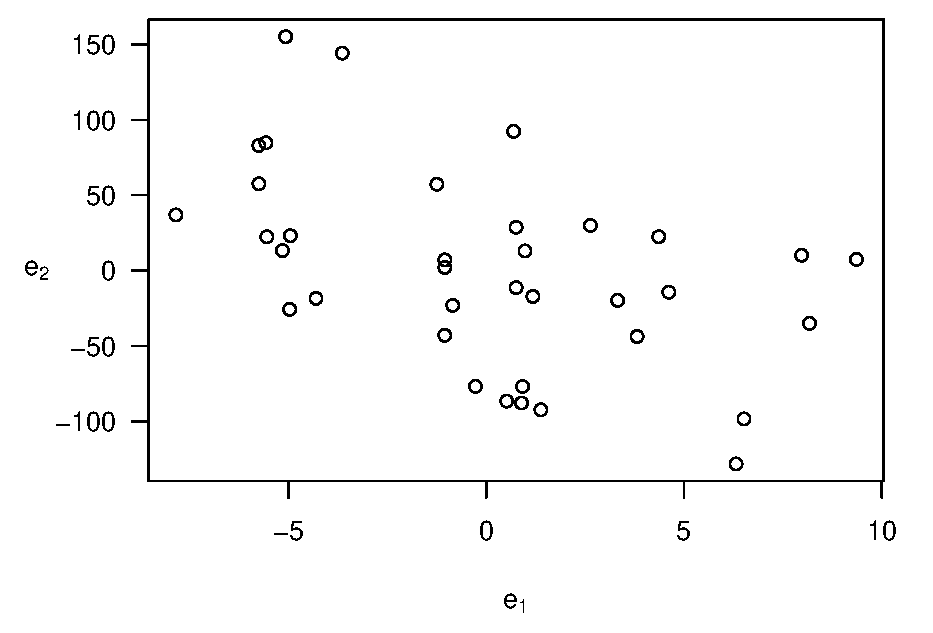
\includegraphics[width=.6\textwidth]{Chapter3/F3RefrigAddedVarPlot.eps}
    \caption{\label{F3:RefrigAddedVarPlot} \small  An added
variable plot. The residuals from the regression of PRICE on the
explanatory variables, omitting ECOST, are on the vertical axis. On
the horizontal axis are the residuals from the regression fit of
ECOST on the other explanatory variables. The correlation
coefficient is -0.48.}
  \end{center}
\end{figure}


The error $\varepsilon $ can be interpreted as the natural variation
in a sample. In many situations, this natural variation is small
compared to the patterns evident in the nonrandom regression
component. Thus, it is useful to think of the error, $\varepsilon_i
= y_i - \left( \beta_0 + \beta_1 x_{i1} + \ldots + \beta_k
x_{ik}\right) $, as the response after controlling for the effects
of the explanatory variables. In Section 3.3, we saw that a random
error can be approximated by a residual, $e_i = y_i - \left( b_0+b_1
x_{i1}+\cdots+b_k x_{ik}\right) $. Thus, in the same way, we may
think of a residual as the response after ``controlling for'' the
effects of the explanatory variables.

With this in mind, we can interpret the vertical axis of Figure
\ref{F3:RefrigAddedVarPlot} as the refrigerator PRICE controlled for
effects of RSIZE, FSIZE, SHELVES and FEATURES. Similarly, we can
interpret the horizontal axis as the ECOST controlled for effects of
RSIZE, FSIZE, SHELVES and FEATURES. The plot then provides a
graphical representation of the relation between PRICE and ECOST,
after controlling for the other explanatory variables. For
comparison, a scatter plot of PRICE and ECOST (not shown here) does
not control for other explanatory variables. Thus, it is possible
that the positive relationship between PRICE and ECOST is not due to
a causal relationship but rather one or more additional variables
that cause both variables to be large.

For example, from Table \ref{T3:RefrigSumStats}, we see that the
freezer size (FSIZE) is positively correlated with both ECOST and
PRICE. It certainly seems reasonable that increasing the size of a
freezer would cause both the energy cost and the price to increase.
Rather, the positive correlation may be due to the fact that large
values of FSIZE mean large values of both ECOST and PRICE.

Variables left out of a regression are called \emph{omitted
variables}. This omission could cause a serious problem in a
regression model fit; regression coefficients could be not only
strongly significant when they should not be, but they may also be
of the incorrect sign. Selecting the proper set of variables to be
included in the regression model is an important task; it is the
subject of Chapters 5 and 6.

\subsection{Partial Correlation Coefficients}\index{correlation coefficients!partial}

As we saw in Chapter 2, a correlation statistic is a useful quantity
for summarizing plots. The correlation for the added variable plot
is called a \emph{partial correlation coefficient}. It is defined to
be the correlation between the residuals $e_1$ and $e_2$ and is
denoted by $ r(y,x_j|x_1,\ldots,x_{j-1},x_{j+1},\ldots,x_k) $.
Because it summarizes an added variable plot, we may interpret $
r(y,x_j|x_1,\ldots,x_{j-1},x_{j+1},\ldots,x_k)$) to be the
correlation between $y$ and $x_j$, in the presence of the other
explanatory variables. To illustrate, the correlation between PRICE
and ECOST in the presence of the other explanatory variables is
-0.48.

The partial correlation coefficient can also be calculated using
\begin{equation}\label{E3:PartialCorr}
r(y,x_j | x_1 ,\ldots, x_{j-1}, x_{j+1}, \ldots, x_k) =
\frac{t(b_j)}{\sqrt{t(b_j)^2 + n-(k+1)}}.
\end{equation}

\noindent Here, $t(b_j)$ is the $t$-ratio for $b_j$ from a
regression of $y$ on $x_1,\ldots,x_k$ (including the variable
$x_j$). An important aspect of equation (\ref{E3:PartialCorr}) is
that it allows us to calculate partial correlation coefficients
running only one regression. For example, from Table
\ref{T3:RefrigFittedModel}, the partial correlation between PRICE
and ECOST in the presence of the other explanatory variables is
$(-3.1)/\sqrt{(-3.1)^2+37-(5+1)}\approx -0.48$.

Calculation of partial correlation coefficients is quicker when
using the relationship with the $t$-ratio, but may fail to detect
nonlinear relationships. The information in Table
\ref{T3:RefrigFittedModel} allows us to calculate all five partial
correlation coefficients in the Refrigerator Price Example after
running only one regression. The three-step procedure for producing
added variable plots requires ten regressions, two for each of the
five explanatory variables. Of course, by producing added variable
plots, we can detect nonlinear relationships that are missed by
correlation coefficients.

Partial correlation coefficients provide another interpretation for
$t$-ratios. Equation (\ref{E3:PartialCorr}) shows how to calculate a
correlation statistic from a $t$-ratio, thus providing another link
between correlation and regression analysis. Moreover, from equation
(\ref{E3:PartialCorr}) we see that the larger is the $t$-ratio, the
larger is the partial correlation coefficient. That is, a large
$t$-ratio means that there is a large correlation between the
response and the explanatory variable, controlling for other
explanatory variables. This provides a partial response to the
question that is regularly asked by consumers of regression
analyses, ``Which variable is most important?''

\section{Some Special Explanatory Variables}

The linear regression model is the basis of a rich family of models.
This section provides several examples to illustrate the richness of
this family. These examples demonstrate the use of (i) binary
variables, (ii) transformation of explanatory variables and (iii)
interaction terms. This section also serves to underscore the
meaning of the adjective \emph{linear} in the phrase ``linear
regression''; the regression function is linear in the parameters
but may be a highly nonlinear function of the explanatory variables.

\marginparjed{The linear regression function is linear in the
parameters but may be a highly nonlinear function of the explanatory
variables.}

\subsection{Binary Variables}\index{explanatory variable!binary}

Categorical variables provide a numerical label for measurements of
observations that fall in distinct groups, or \emph{categories}.
Because of the grouping, categorical variables are discrete and
generally take on a finite number of values. We begin our discussion
with a categorical variable that can take on one of only two values,
a \emph{binary} variable. Further discussion of categorical
variables is the topic of Chapter 4.


\linejed \index{datasets!term life insurance}

\textbf{Example: Term Life Insurance - Continued.} We now consider
the marital status of the survey respondent. In the Survey of
Consumer Finances, respondents can select among several options
describing their marital status including ``married,'' ``living with
a partner,'' ``divorced'' and so on. Marital status is not measured
continuously but rather takes on values that fall into distinct
groups. In this chapter, we group survey respondents according to
whether or not they are single, defined to include those who are
separated, divorced, widowed, never married, and are not married nor
living with a partner. Chapter 4 will present a more complete
analysis of marital status by including additional categories.

\marginparjed{Binary explanatory variables are also known as
indicator and dummy variables.}

The binary variable SINGLE is defined to be one if the survey
respondent is single and 0 otherwise. The variable SINGLE is also
known as an \emph{indicator} variable because it indicates whether
or not the respondent is single. Another name for this important
type of variable is a \emph{dummy} variable. We could use 0 and 100,
or 20 and 36, or any other distinct values. However, 0 and 1 are
convenient for the interpretation of the parameter values, discussed
below. To streamline the discussion, we now present a model using
only LNINCOME and SINGLE as explanatory variables.

\index{plots!letter}

For our sample of $n=275$ households, 57 are single and the other
218 are not.  To see the relationships among LNFACE, LNINCOME and
SINGLE, Figure \ref{F3:LinesLetterPlot} introduces a \emph{letter
plot} of LNFACE versus LNINCOME, with SINGLE as the code variable.
We can see that Figure \ref{F3:LinesLetterPlot} is a scatter plot of
LNFACE versus LNINCOME, using 50 randomly selected households from
our sample of 275 (for clarity of the graph). However, instead of
using the same plotting symbol for each observation, we have coded
the symbols so that we can easily understand the behavior of a third
variable, SINGLE. In other applications, you may elect to use other
plotting symbols such as $\clubsuit , \heartsuit , \spadesuit $, and
so on, or use different colors, to encode additional information.
For this application, the letter codes ``S'' for single and ``o''
for other were selected because they remind the reader of the plot
of the nature of the coding scheme. Regardless of the coding scheme,
the important point is that a letter plot is a useful device for
graphically portraying three or more variables in two dimensions.
The main restriction is that the additional information must be
categorized, such as with binary variables, to make the coding
scheme work.

\begin{figure}[htp]
  \begin{center}
    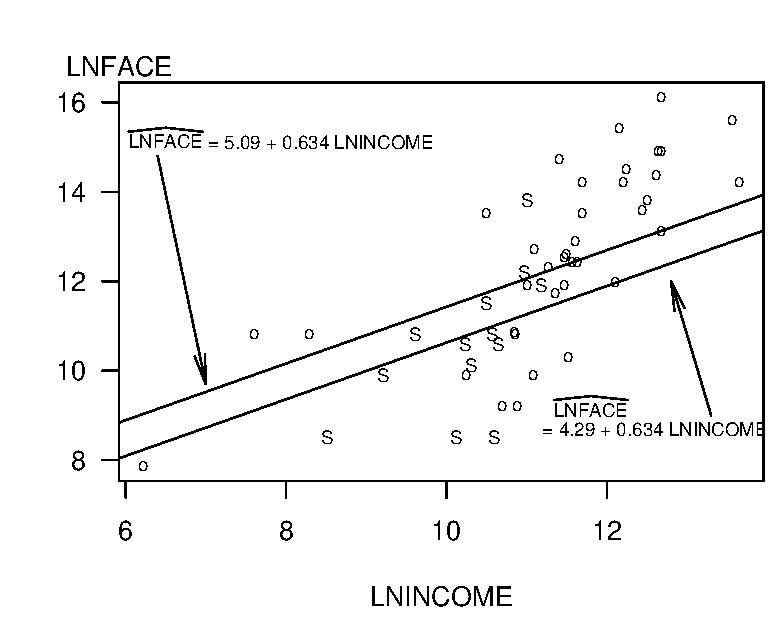
\includegraphics[width=.6\textwidth]{Chapter3/F3LinesLetterPlot.eps}
    \caption{\label{F3:LinesLetterPlot} \small Letter plot of LNFACE versus LNINCOME,
    with the letter code `S'' for single
and ``o'' for other. The fitted regression lines have been
superimposed. The lower line is for single and the upper line is for
other.}
  \end{center}
\end{figure}


Figure \ref{F3:LinesLetterPlot} suggests that LNFACE is lower for
those single than others for a given level of income. Thus, we now
consider a regression model, $LNFACE = \beta_0 + \beta_1 LNINCOME +
\beta_2 SINGLE + \varepsilon$. The regression function can be
written as:

\begin{equation*}
\textrm{E }y = \left\{ \begin{array}{ll}
        \beta_0 + \beta_1  \textrm{LNINCOME}           & \textrm{for other respondents} \\
        \beta_0 + \beta_2 + \beta_1  \textrm{LNINCOME} & \textrm{for single respondents}
\end{array} \right. .
\end{equation*}

The interpretation of the model coefficients differs from the
continuous variable case. For continuous variables such as LNINCOME,
we interpret $\beta_1$ as the expected change in $y$ per unit change
of logarithmic income, holding other variables fixed. For binary
variables such as SINGLE, we interpret $\beta_2$ as the expected
increase in $y$ when going from the base level of SINGLE (=0) to the
alternative level. Thus, although we have one model for both marital
statuses, we can interpret the model using two regression equations,
one for each type of marital status. By writing a separate equation
for each marital status, we have been able to simplify a complicated
multiple regression equation. Sometimes, you will find it easier to
communicate a series of simple relationships compared to a single,
complex relationship.

Although the interpretation for binary explanatory variables differs
from the continuous, the ordinary least squares estimation method
remains valid. To illustrate, the fitted version of the above model
is

\scalefont{0.9}
\begin{center}
\begin{tabular}{cclll}
  $\widehat{LNFACE}$ & = & 5.09   &  + 0.634 LNINCOME & - 0.800 SINGLE .\\
  std error    &   & (0.89) & ~~(0.078) & ~(0.248) \\
\end{tabular}
\end{center}
\scalefont{1.1111}


\noindent To interpret $b_2 = -0.800$, we say that we expect the
logarithmic face to be smaller by 0.80 for a survey respondent who
is single compared to the other category. This assumes that other
things, such as income, remain unchanged. For a graphical
interpretation, the two fitted regression lines are superimposed in
Figure \ref{F3:LinesLetterPlot}.

\linejed

\subsection{Transforming Explanatory Variables}\index{explanatory
variable!transformed}\index{transformations}

Regression models have the ability to represent complex,
\emph{nonlinear} relationships between the expected response and the
explanatory variables. For example, early regression texts, such as
Plackett (1960, Chapter 6) devote an entire chapter of material to
polynomial regression,
\begin{equation}\label{E3:polyregr}
\textrm{E } y  =  \beta_0 + \beta_1 x + \beta_2 x^2 + \ldots +
\beta_p x^p.
\end{equation}

\noindent Here, the idea is that a $p$th order polynomial in $x$ can
be used to approximate general, unknown nonlinear functions of $x$.

The modern day treatment of polynomial regression does not require
an entire chapter because the model in equation (\ref{E3:polyregr})
can be expressed as a special case of the linear regression model.
That is, with the regression function in equation
(\ref{E3:MLRegressionFct}), $\textrm{E } y = \beta_0 + \beta_1 x_1 +
\beta_2 x_2 + \ldots + \beta_k x_k$, we can choose $k = p$ and $x_1
= x, x_2 = x^2, \ldots, x_p = x^p$. Thus, with these choices of
explanatory variables, we can model a highly nonlinear function of
$x$.

We are not restricted to powers of $x$ in our choice of
transformations. For example, the model E $y = \beta_0 + \beta_1 \ln
 x$, provides another way to represent a gently sloping curve in
$x$. This model can be written as a special case of the basic linear
regression model using $x^{\ast} = \ln x$ as the transformed version
of $x$.

Transformations of explanatory variables need not be smooth
functions. To illustrate, in some applications, it is useful to
categorize a continuous explanatory variable. For example, suppose
that $x$ represents the number of years of education, ranging from 0
to 17. If we are relying on information self-reported by our sample
of senior citizens, there may be a substantial amount of error in
the measurement of $x$. We could elect to use a less informative,
but more reliable, transform of $x$ such as $x^{\ast}$, a binary
variable for finishing 13 years of school (finishing high school).
Formally, we would code $x^{\ast}$ = 1 if $x \geq 13$ and $x^{\ast}$
= 0 if $x < 13$.

Thus, there are several ways that nonlinear functions of the
explanatory variables can be used in the regression model. An
example of a nonlinear regression model is $y  =  \beta_0 + \exp
(\beta_1 x) + \varepsilon.$ These typically arise in science
applications of regressions where there are fundamental scientific
principles guiding the complex model development.


\subsection{Interaction Terms}\index{explanatory
variable!interaction}

We have so far discussed how explanatory variables, say $x_1$ and
$x_2$, affect the mean response in an additive fashion, that is, E
$y = \beta_0 + \beta_1 x_1 + \beta_2 x_2$. Here, we expect $y$ to
increase by $\beta_1$ per unit increase in $x_1$, with $x_2$ held
fixed. What if the marginal rate of increase of E $y$ differs for
high values of $x_2$ when compared to low values of $x_2$? One way
to represent this is to create an \emph{interaction variable} $x_3 =
x_1 \times x_2$ and consider the model E $y = \beta_0 + \beta_1 x_1
+ \beta_2 x_2 + \beta_3 x_3$.

With this model, the change in the expected $y$ per unit change in
$x_1$ now depends on $x_2$. Formally, we can assess small changes in
the regression function as

\begin{equation*}
\frac{\partial \textrm{E} y}{\partial x_1} =
\frac{\partial}{\partial x_1} \left(\beta_0 + \beta_1 x_1 + \beta_2
x_2 + \beta_3 x_1 x_2 \right) = \beta_1 + \beta_3 x_2 .
\end{equation*}
In this way, we may allow for more complicated functions of $x_1$
and $x_2$. Figure \ref{F3:Interaction} illustrates this complex
structure. From this figure and the above calculations, we see that
the partial changes of E $y$ due to movement of $x_1$ depend on the
value of $x_2$. In this way, we say that the partial changes due to
each variable are not unrelated but rather ``move together.''


\begin{figure}[htp]
  \begin{center}
    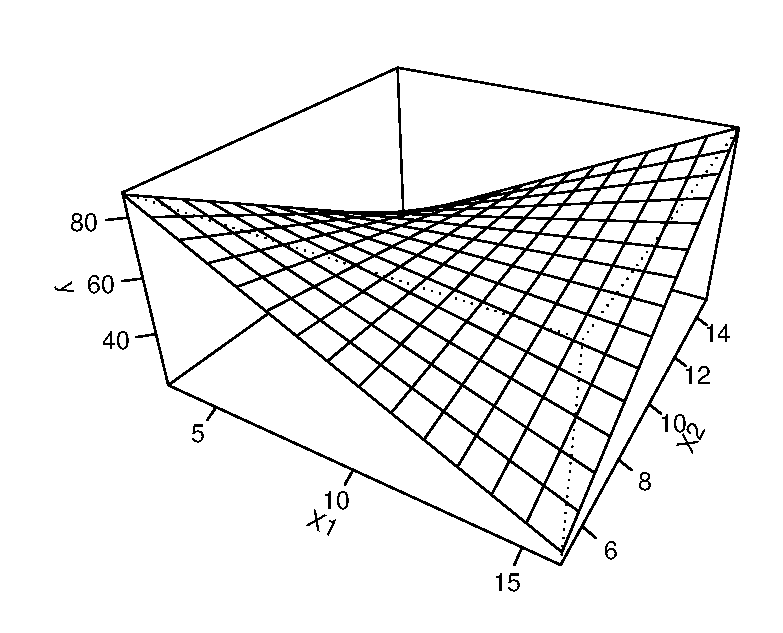
\includegraphics[width=.6\textwidth]{Chapter3/F3Interaction.eps}
    \caption{\label{F3:Interaction} \small Plot of E $y = \beta_0 +
         \beta_1 x_1 + \beta_2 x_2 + \beta_3 x_1 x_2$ versus $x_1$ and
          $x_2$.}
  \end{center}
\end{figure}

More generally, an interaction term is a variable that is created as
a nonlinear function of two or more explanatory variables. These
special terms, even though permitting us to explore a rich family of
nonlinear functions, can be cast as special cases of the linear
regression model. To do this, we simply create the variable of
interest and treat this new term as another explanatory variable. Of
course, not every variable that we create will be useful. In some
instances, the created variable will be so similar to variables
already in our model that it will provide us with no new
information. Fortunately, we can use $t$-tests to check whether the
new variable is useful. Further, Chapter 4 will introduce a test to
decide whether a group of variables is useful.

The function that we use to create an interaction variable must be
more than just a linear combination of other explanatory variables.
For example, if we use $x_3 = x_1 + x_2$, we will not be able to
estimate all of the parameters. Chapter 5 will introduce some
techniques to help avoid situations when one variable is a linear
combination of the others.

To give you some exposure to the wide variety of potential
applications of special explanatory variables, we now present a
series of short examples.

\bigskip

\linejed

\textbf{Example: Term Life Insurance - Continued.} How do we
interpret the interaction of a binary variable with a continuous
variable? To illustrate, consider a Term Life regression model,
$\textrm{LNFACE} = \beta_0 + \beta_1 \textrm{LNINCOME} + \beta_2
\textrm{SINGLE} + \beta_2 \textrm{LNINCOME*SINGLE} + \varepsilon$.
In this model, we have created a third explanatory variable through
the interaction of LNINCOME and SINGLE. The regression function can
be written as:
\begin{equation*}
\textrm{E }y = \left\{ \begin{array}{ll}
        \beta_0 + \beta_1  \textrm{LNINCOME}           & \textrm{for other respondents} \\
        \beta_0 + \beta_2 + (\beta_1 + \beta_3)  \textrm{LNINCOME} & \textrm{for single respondents}
\end{array} \right. .
\end{equation*}
Thus, through this single model with four parameters, we can create
two separate regression lines, one for those single and one for
others. Figure \ref{F3:LetterInteract} shows the two fitted
regression lines for our data.


\begin{figure}[htp]
  \begin{center}
    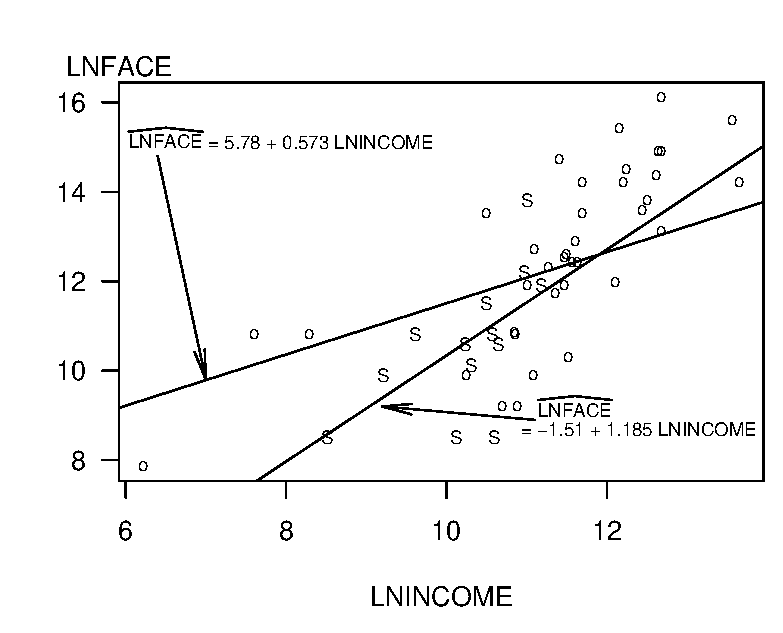
\includegraphics[width=0.6\textwidth]{Chapter3/F3LetterInteract.eps}
    \caption{\label{F3:LetterInteract} \small Letter plot of LNFACE versus LNINCOME,
    with the letter code `S'' for single
and ``o'' for other. The fitted regression lines have been
superimposed. The lower line is for single and the upper line is for
other.}
  \end{center}
\end{figure}

\linejed \index{examples!life insurance company expenses}

\textbf{Example: Life Insurance Company Expenses.}\ecaptionjed{Life
Insurance Company Expenses} In a well-developed life insurance
industry, minimizing expenses is critical for a company's
competitive position. Segal (2002) analyzed annual accounting data
from over 100 firms for the period 1995-1998, inclusive, using a
data base from the National Association of Insurance Commissioners
(NAIC) and other reported information. Segal modeled overall company
expenses as a function of firm outputs and the price of inputs. The
outputs consist of insurance production, measured by $x_1$ through
$x_5$, described in Table \ref{T3:Expenses}. Segal also considered
the square of each output, as well as an interaction term with a
dummy/binary variable $D$ that indicates whether or not the firm
uses a branch company to distribute its products. (In a branch
company, field managers are company employees, not independent
agents.)\index{actuarial \& financial terms and concepts!insurance
company branch office}

\scalefont{0.9}
\begin{center}  \begin{table}[h] \caption{\label{T3:Expenses}
Twenty-Three Regression Coefficients from an Expense Cost Model}
\begin{tabular}{l|rrrr}
\hline
 &  \multicolumn{2}{c}{Variable} &  \multicolumn{2}{c}{Variable
 Squared} \\
  &  Baseline &  Interaction  &  Baseline &  Interaction \\
  &   &   with~~   &   &   with~~  \\
Variable & $(D=0)$ &  $(D=1)$ & $(D=0)$ &  $(D=1)$\\
\hline Number of Life Policies Issued ($x_1$)     &  -0.454 & 0.152
& 0.032
& -0.007 \\
Amount of Term Life Insurance Sold ($x_2$)  & 0.112 & -0.206 & 0.002
& 0.005 \\
Amount of Whole Life Insurance Sold ($x_3$) & -0.184 & 0.173 & 0.008
& -0.007 \\
Total Annuity Considerations ($x_4$)        & 0.098 & -0.169 &
-0.003 & 0.009 \\
Total Accident and Health Premiums ($x_5$)  &-0.171 & 0.014 & 0.010
& 0.002 \\
Intercept  & 7.726 & & & \\
Price of Labor (PL) & 0.553 & & & \\
Price of Capital (PC) & 0.102 & & & \\
\hline
\end{tabular}
\newline
\flushleft ~~~Note: $x_1$ through $x_5$ are in logarithmic units.
\textit{Source: Segal (2002)}
\end{table}  \end{center}  \scalefont{1.1111}
For the price inputs, the price of labor ($PL$) is defined to be the
total cost of employees and agents divided by their number, in
logarithmic units. The price of capital ($PC$) is approximated by
the ratio of capital expense to the number of employees and agents,
also in logarithmic units. The price of materials consists of
expenses other than labor and capital divided by the number of
policies sold and terminated during the year. It does not appear
directly as an explanatory variable. Rather, Segal took the
dependent variable ($y$) to be total company expenses divided by the
price of materials, again in logarithmic units.

With these variable definitions, Segal estimated the following
regression function.
\begin{equation*}
\mathrm{E~}y=\beta_0 + \sum_{j=1}^5 \left( \beta_j x_j + \beta_{j+5}
D x_j + \beta_{j+10} x_j^2 + \beta_{j+15}D x_j^2  \right) +
\beta_{21} PL + \beta_{22} PC.
\end{equation*}
The parameter estimates appear in Table \ref{T3:Expenses}. For
example, the marginal change in E $y$ per unit change in $x_1$ is
\begin{equation*}
\frac{\partial ~ \mathrm{E}y}{\partial x_1}= \beta_1 + \beta_{6} D +
2 \beta_{11} x_1 + 2 \beta_{16}D x_1,
\end{equation*}
which is estimated as $ -0.454 + 0.152 D + (0.064 - 0.014 D) x_1$.
For these data, the median number of policies issued was
$x_1=15,944$. At this value of $x_1$, the estimated marginal change
is $ -0.454 + 0.152 D + (0.064 - 0.014 D) \mathrm{ln}(15944) = 0.165
+ 0.017 D,$ or 0.165 for baseline $(D=0)$ and 0.182 for branch
$(D=1)$ companies.

These estimates are elasticities, as defined in Section 3.2.2. To
interpret these coefficients further, let $COST$ represent total
general company expenses and $NUMPOL$ represent the number of life
policies issued. Then, for branch $(D=1)$ companies, we have
\begin{equation*}
0.182 \approx \frac{\partial y }{\partial x_1 } = \frac{\partial ~
\mathrm{ln}~COST}{\partial ~ \mathrm{ln}~NUMPOL}= \frac{
\frac{\partial ~ COST}{\partial ~NUMPOL}} {\frac{COST}{NUMPOL}},
\end{equation*}
or $\frac{\partial ~ COST}{\partial ~NUMPOL} \approx 0.182
\frac{COST}{NUMPOL}$. The median cost is \$15,992,000, so the
marginal cost per policy at these median values is $ 0.182 \times
(15992000/15944) = \$182.55$.

\linejed


\bigskip

\textbf{Special Case: Curvilinear Response Functions}. We can expand
the polynomial functions of an explanatory variable to include
several explanatory variables. For example, the expected response,
or \emph{response function}, for a second-order model with two
explanatory variables is\index{response function}

\begin{equation*}
\textrm{E} y = \beta_0 + \beta_1 x_1 + \beta_2 x_2 + \beta_{11}
x_1^2 + \beta_{22} x_2^2 + \beta_{12} x_1 x_2.
\end{equation*}


Figure \ref{F3:Curvilinear} illustrates this response function.
Similarly, the response function for a second-order model with three
explanatory variables is

\begin{equation*}
\textrm{E} y = \beta_0 + \beta_1 x_1 + \beta_2 x_2 + \beta_3 x_3 +
\beta_{11} x_1^2 + \beta_{22} x_2^2 + \beta_{33} x_3^2 + \beta_{12}
x_1 x_2 + \beta_{13} x_1 x_3 + \beta_{23} x_2 x_3.
\end{equation*}

When there is more than one explanatory variable, third and higher
order models are rarely used in applications.


\begin{figure}[htp]
  \begin{center}
    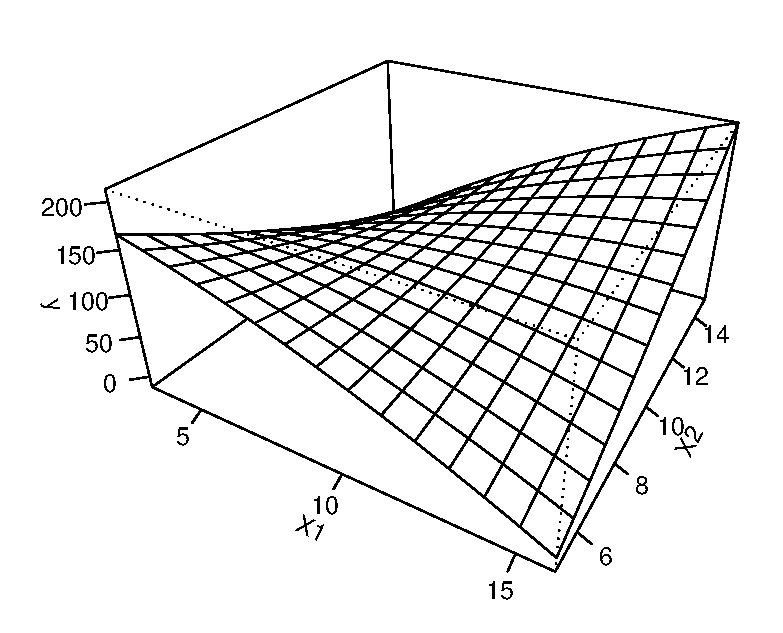
\includegraphics[width=.6\textwidth]{Chapter3/F3Curvilinear.eps}
    \caption{\label{F3:Curvilinear} \small Plot of E $y = \beta_0 + \beta_1 x_1 + \beta_2 x_2 +
     \beta_{11} x_1^2 + \beta_{22} x_2^2 + \beta_{12} x_1 x_2$ versus
$x_1$ and $x_2$.}
  \end{center}
\end{figure}

\bigskip

\textbf{Special Case: Nonlinear Functions of a Continuous Variable}.
In some applications, we expect the response to have some abrupt
changes in behavior at certain values of an explanatory variable,
even if the variable is continuous. For example, suppose that we are
trying to model an individual's charitable contributions ($y$) in
terms of their wages ($x$). For 2007 data, a simple model we might
entertain is given in Figure \ref{F3:Charity}.


\begin{figure}[htp]
  \begin{center}
    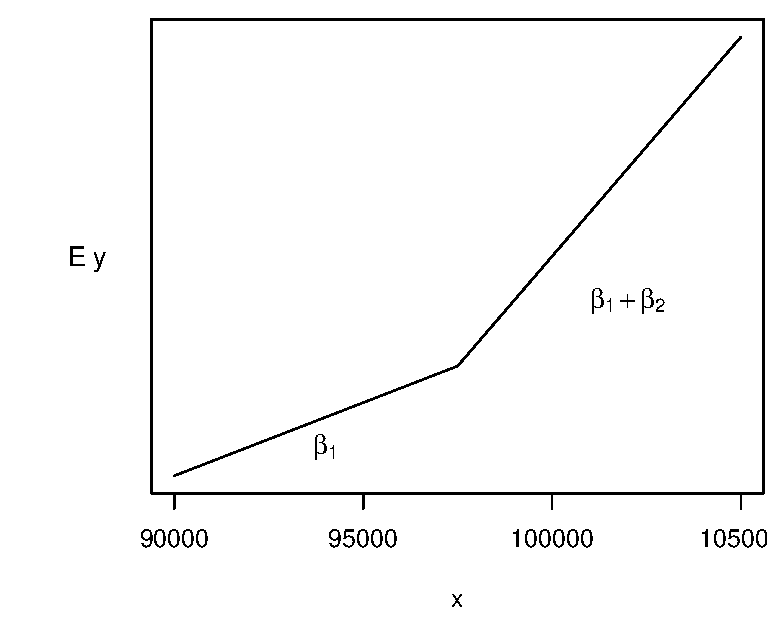
\includegraphics[width=.6\textwidth]{Chapter3/F3Charity.eps}
    \caption{\label{F3:Charity} \small The marginal change in E $y$ is
    lower below \$97,500. The parameter $\beta_2$ represents the
    difference in the slopes.}
  \end{center}
\end{figure}


A rational for this model is that, in 2007 individuals paid 7.65\%
of their income for Social Security taxes up to \$97,500. No social
security taxes are excised on wages in excess of \$97,500. Thus, one
theory is that, for wages in excess of \$97,500, individuals have
more disposal income per dollar and thus should be more willing to
make charitable contributions.

To model this relationship, define the binary variable $z$ to be
zero if $x < 97,500$ and to be one if $x \geq  97,500$. Define the
regression function to be E $y = \beta_0 + \beta_1 x + \beta_2 z (x
- 97,500).$ This can be written as:


\begin{equation*}
\textrm{E }y = \left\{ \begin{array}{ll}
        \beta_0 + \beta_1  x                    & x < 97,500 \\
        \beta_0 - \beta_2(97,500) + (\beta_1+\beta_2) x & x \geq  97,500
\end{array} . \right.
\end{equation*}

\noindent To estimate this model, we would run a regression of $y$
on two explanatory variables, $x_1 = x$ and $x_2 = z \times (x -
97,500)$. If $\beta_2 > 0,$ then the marginal rate of charitable
contributions is higher for incomes exceeding \$97,500.

Figure \ref{F3:Charity} illustrates this relationship, known as
\emph{piecewise linear regression} or sometimes a ``broken stick''
model. The sharp break in Figure \ref{F3:Charity} at $x = 97,500$ is
called a ``kink.'' We have linear relationships above and below the
kinks and have used a binary variable to put the two pieces
together. We are not restricted to one kink. For example, suppose
that we wish to do a historical study of Federal taxable income for
1992 single filers. Then, there were three tax brackets: the
marginal tax rate below \$21,450 was 15\%, above \$51,900 was 31\%,
and in between was 28 percent. For this example, we would use two
kinks, at 21,450 and 51,900.\index{regression model!piecewise
linear}\index{regression model!broken stick}

Further, piecewise linear regression is not restricted to continuous
response functions. For example, suppose that we are studying the
commissions paid to stockbrokers ($y$) in terms of the number of
shares purchased by a client ($x$). We might expect to see the
relationship illustrated in Figure \ref{F3:Break}. Here, the
discontinuity at $x = 100$ reflects the administrative expenses of
trading in odd lots, as trades of less than 100 shares are called.
The lower marginal cost for trades in excess of 100 shares simply
reflects the economies of scale for doing business in larger
volumes. A regression model of this is E $y = \beta_0 + \beta_1 x +
\beta_2 z + \beta_3 z x$ where $z = 0$ if $x < 100$ and $z = 1$ if
$x \geq 100$. The regression function depicted in Figure
\ref{F3:Break} is

\begin{equation*}
\textrm{E }y = \left\{ \begin{array}{ll}
        \beta_0 + \beta_1  x_1                    & x<100 \\
        \beta_0 + \beta_2 + (\beta_1+\beta_3) x_1 & x \geq 100
\end{array} . \right.
\end{equation*}

\begin{figure}[htp]
  \begin{center}
    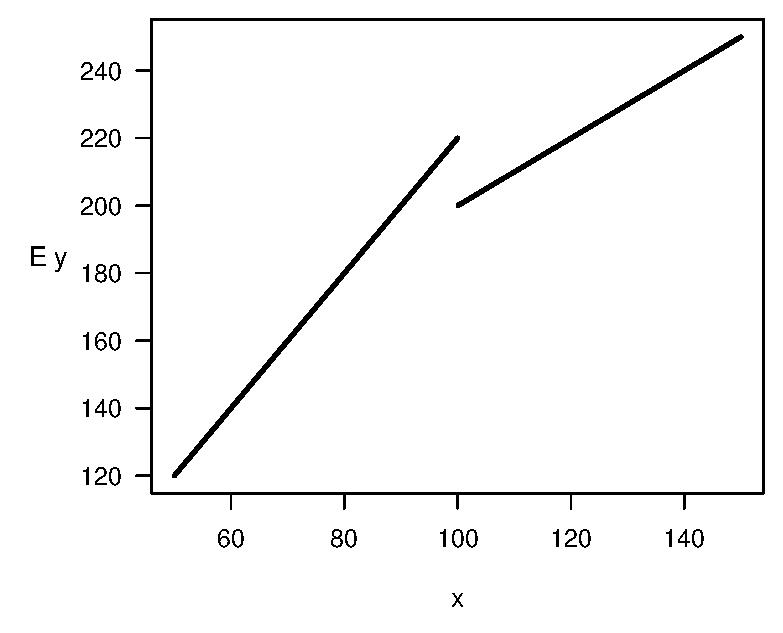
\includegraphics[width=.6\textwidth]{Chapter3/F3Break.eps}
    \caption{\label{F3:Break} \small Plot of expected commissions (E $y$) versus number of shares traded ($x$).
    The break at $x=100$ reflects savings in administrative expenses.
    The lower slope for $x \geq 100$ reflects economies of scales in expenses.}
  \end{center}
\end{figure}


\section{Further Reading and References}

For proofs of the Chapter 3 results, we refer the reader to
Goldberger (1991). Nonlinear regression models are discussed in, for
example, Bates and Watts (1988).

Chapter 3 has introduced the fundamentals of multiple linear
regression. Chapter 4 will widen the scope by introducing
categorical variables and statistical inference methods for handling
several coefficients simultaneously. Chapter 5 will introduce
techniques to help you pick appropriate variables in a multiple
linear regression model. Chapter 6 is a synthesis chapter,
discussing model interpretation, variable selection and data
collection.

\bigskip


\textbf{Chapter References}

\begin{multicols}{2}

\scalefont{0.9}

Bates, Douglas M. and Watts, D. G. (1988). \textit{Nonlinear
Regression Analysis and its Applications}. John Wiley \& Sons, New
York.

Lemaire, Jean (2002). Why do females live longer than males?
\textit{North American Actuarial Journal} 6(4), 21-37.

Goldberger, Arthur (1991). \textit{A Course in Econometrics}.
Harvard University Press, Cambridge.

Plackett, R.L. (1960). \textit{Regression Analysis}. Clarendon
Press, Oxford, England.

Segal, Dan (2002). An economic analysis of life insurance company
expenses. \textit{North American Actuarial Journal} 6(4), 81-94.

\scalefont{1.1111}

\end{multicols}

\bigskip


\section{Exercises}

\begin{exercises}

\scalefont{0.90}

\item  Consider a fictitious data set of $n = 100$ observations with
$s_y = 80$. We run a regression with three explanatory variables to
get $s = 50$.

a.  Calculate the adjusted coefficient of determination, $R_a^2$.

b. Complete the ANOVA table.

\begin{center}
\begin{tabular}{l|lcl}
\hline \multicolumn{4}{c}{ANOVA\ Table} \\ \hline Source & Sum of
Squares & $df$ & Mean Square \\ \hline
Regression & &  & \\
Error &  &  &  \\
Total &  &  &  \\ \hline
\end{tabular}
\end{center}

c.  Calculate the (unadjusted) coefficient of determination, $R^2$.

\item  Consider a fictitious data set of $n = 100$
observations with $s_y = 80$. We run a regression with three
explanatory variables to get $s = 50$. We also get
\begin{equation*}
\left(\mathbf{X^{\prime} X} \right)^{-1} = \left(
\begin{array}{cccc}
100 & 20 &20 & 20\\
20 & 90 & 30 & 40 \\
20 & 30 & 80 & 50 \\
20 & 40 & 50 & 70 \\
\end{array}
\right).
\end{equation*}

a. Determine the standard error of $b_3$, $se(b_3)$.

b. Determine the estimated covariance between $b_2$ and $b_3$.

c. Determine the estimated correlation between $b_2$ and $b_3$.

d. Determine the estimated variance of $4b_2 + 3b_3$.

\item Consider the following small fictitious data set. You will be
fitting a regression model to $y$ using two explanatory variables,
$x_1$ and $x_2$.

\begin{center}
\begin{tabular}{c|cccc}
\hline $i$ & 1 & 2 & 3 & 4 \\
$x_{i,1}$ & -1 & 2 & 4 & 6 \\
$x_{i,2}$ & 0 & 0 & 1 & 1 \\
$y_i$ & 0 & 1 & 5 & 8 \\
 \hline
\end{tabular}
\end{center}

\noindent From the fitted regression model, we have $s = 1.373$ and
\begin{equation*}
\mathbf{b} = \left(
\begin{array}{c}
0.15 \\ 0.692 \\2.88
\end{array}
\right) ~~~\mathrm{and}~~~ \left(\mathbf{X^{\prime} X} \right)^{-1}
= \left(
\begin{array}{cccc}
0.53846 & -0.07692 &-0.15385\\
-0.07692 & 0.15385 & -0.69231 \\
-0.15385 & -0.69231 & 4.11538 \\
\end{array}
\right).
\end{equation*}

a. Write down the vector of dependent variables, $\mathbf{y}$, and
the matrix of explanatory variables, $\mathbf{X}$.

b. Determine the numerical value for $\widehat{y}_3$, the fitted
value for the third observation.

c. Determine the numerical value for $se(b_2)$.

d. Determine the numerical value for $t(b_1)$.

\empexjed{WiscLottery}\index{datasets!Wisconsin lottery sales}

\item \textbf{Wisconsin Lottery.}\label{Ex:Lottery3}
Section 2.1 described a sample of $n=50$ geographic areas (zip
codes) containing sales data on the Wisconsin state lottery ($y =
SALES$). In that section, sales were analyzed using a basic linear
regression model with $x = POP$, the area population, as the
explanatory variable. This exercise extends that analysis by
introducing additional explanatory variables given in Table
\ref{Ex:LotVariables}.


\begin{table}[h]
\scalefont{0.8}
 \caption{\label{Ex:LotVariables} \small Lottery,
economic and demographic characteristics of fifty Wisconsin ZIP
codes}
\begin{center}
\begin{tabular}{ll}
\hline
\multicolumn{ 2}{c}{{\bf Lottery characteristics}} \\
  SALES  & Online lottery sales to individual consumers \\
\hline
\multicolumn{ 2}{c}{{\bf Economic and demographic characteristics}} \\
 PERPERHH  & Persons per household  \\
 MEDSCHYR  & Median years of schooling  \\
   MEDHVL  & Median home value in \$1000s for owner-occupied homes \\
 PRCRENT   & Percent of housing that is renter occupied \\
 PRC55P    & Percent of population that is 55 or older \\
 HHMEDAGE  & Household median age \\
MEDINC      & Estimated median household income, in \$1000s \\
POP   & Population, in thousands \\
\hline

\end{tabular}
\scalefont{1.25}
\end{center}
\end{table}

a. Produce a table of summary statistics for all variables. One zip
code (observation 11, zip = 53211, Shorewood Wisconsin a suburb of
Milwaukee) appears to have unusually large values of MEDSCHYR and
MEDHVL. For this observation, how many standard deviations is the
value of MEDSCHYR above the mean? For this observation, how many
standard deviations is the value of MEDHVL above the mean?

b. Produce a table of correlations. What three variables are most
highly correlated with SALES?

c. Produce a scatter plot matrix of all explanatory variables and
SALES. In the plot of MEDSCHYR versus SALES, describe the position
of observation 11.

d. Fit a linear model of SALES on all eight explanatory variables.
Summarize the fit of this model by citing the residual standard
deviation, $s$, the coefficient of determination, $R^2$ and its
adjusted version, $R^2_a$.

e. Based on your part (d) model fit, is MEDSCHYR a statistically
significant variable? To respond to this question, use a formal test
of hypothesis. State your null and alternative hypotheses, decision
making criterion and your decision-making rule.

f. Now fit a more parsimonious model, using SALES as the dependent
variable and MEDSCHYR, MEDHVL and POP as explanatory variables.
Summarize the fit of this model by citing the residual standard
deviation, $s$, the coefficient of determination, $R^2$ and its
adjusted version, $R^2_a$. How do these values compare to the model
fit in part (d)?

g. Note that the sign of the regression coefficient associated with
MEDSCHYR is now negative. To help interpret this coefficient,
compute the corresponding partial correlation coefficient. What is
the interpretation of this coefficient.

h. To get further insights into the relation between MEDSCHYR and
SALES, produce an added variable plot controlling for the effects of
MEDHVL and POP. Check that the correlation associated with this plot
agrees with your answer in part (g).

i. Re-run the regression in part (f), after removing observation 11.
Cite the basic summary statistics from this regression. For this
model fit, is MEDSCHYR a statistically significant variable? To
respond to this question, use a formal test of hypothesis. State
your null and alternative hypotheses, decision making criterion and
your decision-making rule.

j. Re-run the regression in part (f), after removing observation 9.
Cite the basic summary statistics from this regression.

\empexjed{NAICExpense}\index{datasets!insurance company expenses}

\item \textbf{Insurance company expenses.}\label{Ex:NAICExpense3}
This exercise considers insurance company data from the NAIC and
described in Exercise 1.\ref{Ex:NAICExpense}.

Table \ref{Ex:NAICVariables} describes several variables that can be
used to explain expenses. As with Segal's (2002) study of life
insurers, firm ``outputs'' consist of premiums written (for property
and casualty, these are subdivided into personal and commercial
lines) as well as losses (subdivided into short and long tail
lines). ASSETS and CASH are commonly used measures of the size of a
company. GROUP, STOCK and MUTUAL describe the organizational
structure. Firm ``inputs'' were gathered from the Bureau of Labor
Statistics (BLS, from the Occupational Employee Statistics program).
WAGESTAFF is calculated as the average wage in the state where the
insurance company headquartered. AGENTWAGE is calculated as the
weighted average of annual wages of the brokerage industry, weighted
by the percentage of gross premium written in each state.




\begin{table}[h]
\scalefont{0.8} \caption{\label{Ex:NAICVariables} \small Insurer
Expense Variables}
\begin{tabular}{l|l}
\hline
\bf Variable & \multicolumn{1}{c} {\bf Description} \\
\hline
\multicolumn{2}{c} {\bf NAIC Variables } \\
\hline
EXPENSES & Total expenses incurred, in millions of dollars \\
    LOSSLONG & Losses incurred for long tail lines, in millions of dollars \\
    LOSSSHORT& Losses incurred for short tail lines, in millions of dollars \\
GPWPERSONAL & Gross premium written for personal lines, in millions of dollars \\
  GPWCOMM  & Gross premium written for commercial lines, in millions of dollars \\
ASSETS & Net admitted assets, in millions of dollars \\
CASH & Cash and invested assets, in millions of dollars \\
      GROUP & Indicates if the company is affiliated  \\
      STOCK & Indicates if the company is a stock company \\
     MUTUAL & indicates if the company is a mutual company \\
\hline \multicolumn{2}{c} {\bf BLS Variables } \\ \hline
STAFFWAGE & Annual average wage of the insurer's administrative staff,  \\
 & ~~~~in thousands of dollars  \\
AGENTWAGE & Annual average wage of the insurance agent, in thousands of dollars \\
\hline

\end{tabular}
\scalefont{1.25}
\end{table}

\bigskip

A preliminary inspection of the data showed that many firms did not
report any insurance losses incurred in 2005. For this exercise, we
consider the 384 companies with some losses in the file
``NAICExpense.csv''.

a. Produce summary statistics of the response variable and the
(non-binary) explanatory variables. Note the pattern of skewness for
each variable. Note that many variables have negative values.

b. Transform each non-binary variable through the modified logarithm
transform, $\ln(1+x)$. Produce summary statistics of these modified
non-binary explanatory variables. Let LNEXPENSES
($=\ln(1+EXPENSES)$) denote the modified expense variable.

For subsequent analysis, use only the modified variables described
in part (b).

c. Produce a table of correlations for the non-binary variables.
What three variables are most highly correlated with LNEXPENSES?

d. Provide a boxplot of LNEXPENSES by level of GROUP. Which level of
group has higher expenses?

e. Fit a linear model of LNEXPENSES on all eleven explanatory
variables. Summarize the fit of this model by citing the residual
standard deviation, $s$, the coefficient of determination, $R^2$ and
its adjusted version, $R^2_a$.

f. Fit a linear model of LNEXPENSES on a reduced model using eight
explanatory variables, dropping CASH, STOCK and MUTUAL. For the
explanatory variables, include assets, GROUP, both versions of
losses and gross premiums, as well as the two BLS variables.

f(i). Summarize the fit of this model by citing $s$, $R^2$ and
$R^2_a$.

f(ii). Interpret the coefficient associated with commercial lines
gross premiums on the logarithmic scale.

f(iii). Suppose that GPWCOMM increases by \$1, how much do we expect
EXPENSES to increase? Use your answer in part f(ii) and median
values of GPWCOMM and EXPENSES for this question.

g. Square each of the two loss and the two gross premium variables.
Fit a linear model of LNEXPENSES on a reduced model using twelve
explanatory variables, the eight variables in part (f) and the four
additional squared terms just created.

g(i). Summarize the fit of this model by citing  $s$,  $R^2$ and
$R^2_a$.

g(ii). Do the quadratic variables appear to be useful explanatory
variables?\index{explanatory variable!quadratic}


h. Now omit the two BLS variables, so you are fitting a model of
LNEXPENSES on assets, GROUP, both versions of losses and gross
premiums, as well as quadratic terms. Summarize the fit of this
model by citing $s$, $R^2$ and $R^2_a$. Comment on the number of
observations used to fit this model compared to part (f).

i. Drop the quadratic terms in part (g) and add interaction terms
with the dummy variable GROUP. Thus, there are now eleven variables,
assets, GROUP, both versions of losses and gross premiums, as well
as interactions of GROUP with assets and both versions of losses and
gross premiums.

i(i). Summarize the fit of this model by citing $s$, $R^2$ and
$R^2_a$.

i(ii). Suppose that GPWCOMM increases by \$1, how much do we expect
EXPENSES to increase for GROUP=0 companies? Use the median values of
GPWCOMM and EXPENSES of GROUP=0 companies for this question.

i(iii). Suppose that GPWCOMM increases by \$1, how much do we expect
EXPENSES to increase for GROUP=1 companies? Use the median values of
GPWCOMM and EXPENSES of GROUP=1 companies for this question.

\empexjed{UNLifeExpectancy}\index{datasets!national life
expectancies}

\item \textbf{National Life Expectancies.}\label{Ex:UNLIFE3} We
continue the analysis begun in Exercises 1.\ref{Ex:UNLIFE} and
2.\ref{Ex:UNLIFE2}. Now fit a regression model on LIFEEXP using
three explanatory variables, FERTILITY, PUBLICEDUCATION and lnHEALTH
(the natural logarithmic transform of PRIVATEHEALTH).

a. Interpret the regression coefficient associated with public
education.

b. Interpret the regression coefficient associated with health
expenditures without using the logarithmic scale for expenditures.

c. Based on the model fit, is PUBLICEDUCATION a statistically
significant variable? To respond to this question, use a formal test
of hypothesis. State your null and alternative hypotheses,
decision-making criterion and your decision-making rule.

d. The negative sign of the PUBLICEDUCATION coefficient is
surprising, in that the sign of the correlation between
PUBLICEDUCATION and LIFEEXP is positive and intuition suggests a
positive relation. To check this result, an added variable plot
appears in Figure~\ref{Ex:UNLIFEPlot2}.

d(i). For an added variable plot, describe its purpose and a method
for producing it.

d(ii). Calculate the correlation corresponding to the added variable
plot that appears in Figure~\ref{Ex:UNLIFEPlot2}.

\begin{figure}[htp]
  \begin{center}
   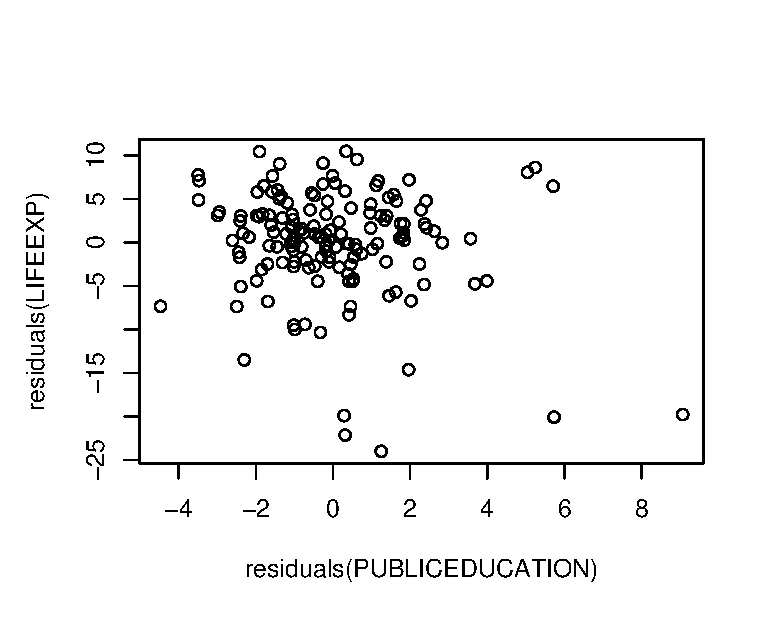
\includegraphics[width=.6\textwidth]{Chapter3/UNLIFE2.eps}
   \caption{\label{Ex:UNLIFEPlot2} \small  Added variable plot of PUBLICEDUCATION  versus LIFEEXP,
   controlling for FERTILITY and lnHEALTH.}
  \end{center}
\end{figure}


\scalefont{1.1111}
\end{exercises}
